\chapter{Edward Sapir}
\label{ch.sapir}

As observed in the preceding chapter, {\Boas} continued to play a leading
role in the development of American linguistics right up until his
death in 1942. His influence was exerted through his direction of
various funding agencies and organs of publication and, more
generally, by his approving and encouraging (or withholding such
support from) the work of other scholars. It was, for example, partly
because of {\Boas}'s `patronage' that \name{Roman}{Jakobson} was able to
establish himself in the United States within a relatively short time
after his arrival, as noted in chapter~\ref{ch.jakobson} above.

In substantive terms, however, {\Boas}'s influence on the development of
linguistic theory in America was rather indirect in the years
following the publication of the first volume of the \textsl{Handbook
  of American Indian Languages} \citep{boas:handbook_1}. Though his
basic tenets continued to shape the orientation of linguistic research
and to form the basis of a developing American approach to the science
of language, he did not himself play a leading role in the formation
of linguistic theory. This was not just because, as described in
detail by \citet[ch. 3]{murray93:theory.groups}, he was averse to
theory but also because his own interests were largely elsewhere: in
the more general field of \isi{ethnography}, not only linguistics; and
within linguistics, in the description of the native languages of
North America. It thus fell largely to {\Boas}'s students, proceeding
from his general views, to develop a more specific and articulated
theory of linguistic structure. By far the most important among {\Boas}'s
students in this respect was \name{Edward}{Sapir}, who had substantially
eclipsed {\Boas} as a theoretician of language by the mid-1920s.

\section{Sapir's life}

\name{Edward}{Sapir} was born in 1884 in Lauenburg,
Germany.\footnote{\citet{darnell90:sapir} provides an extensive and
  detailed account of {\Sapir}'s life and career, though reservations may
  be necessary on some points, as suggested by
  \citet{silverstein91:rvw.darnell}. \citealt{cowan.etal86:sapir.centennial}
  represents the content of a symposium in 1984 on the occasion of the
  centennial of {\Sapir}'s birth. \citealt{koerner84:sapir.appraisals} is
  a collection of articles about {\Sapir}'s life and work, issued on that
  occasion.} When he was five, his parents emigrated to the United
States, where he attended school in New York. He received a BA from
Columbia in 1904, and went on to earn a master's degree there in 1905
in Germanics with a minor in {Sanskrit}. While at Columbia he met and
began to study with {\Boas}; in the years immediately following his MA he
did fieldwork in the state of Washington on the Wishram dialect of
Chinook, and in Oregon on {Takelma} with Mrs. \name{Frances}{Johnson}, under
{\Boas}'s guidance. In 1907-8 he was a research associate in \isi{anthropology}
at the University of California (Berkeley) under \name{Alfred}{Kroeber}, where
he worked on Yana.

\begin{wrapfigure}{r}{.4\textwidth}
  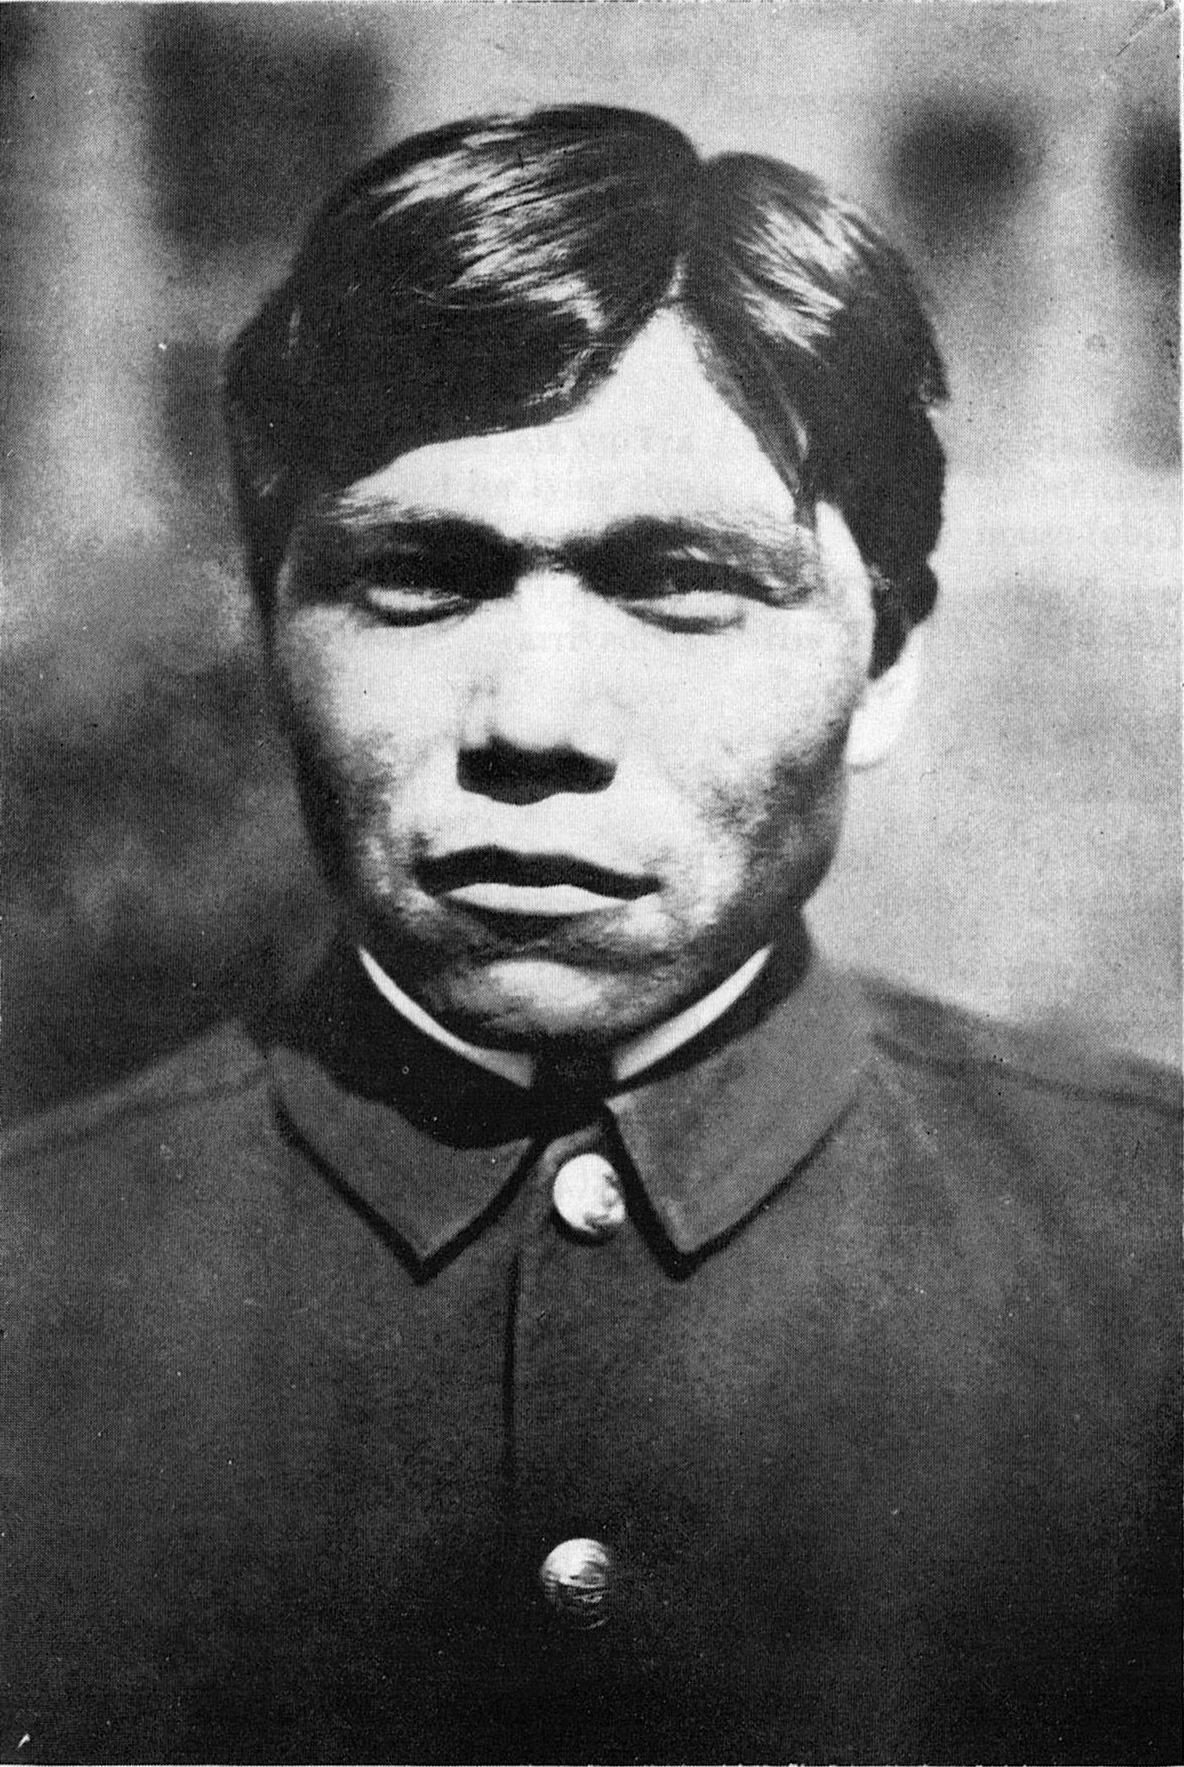
\includegraphics[width=.95\textwidth]{figures/tillohash.jpg}
  \caption{Tony Tillohash, Kaibab Paiute Indian, in his Carlisle
    School Uniform}
  \label{fig:ch.sapir.tillohash}
\end{wrapfigure}
This was followed by two years' appointment at the University of
Pennsylvania in Philadelphia, as a fellow and subsequently as
instructor. During this period (with the support of the University of
Pennsylvania Museum) he had a {Southern Paiute} student, \name{Tony}{Tillohash}\footnote{\citet{fowler86:tillohash} provide a fuller picture
  of \name{Tony}{Tillohash}'s background and life after his work with {\Sapir},
  and the relation of that work to {\Sapir}'s analyses of Southern
  Paiute.}  from the Carlisle Indian School, to work with in
Philadelphia, and did fieldwork in the summer of 1909 with Utes on the
Uintah Reservation in Utah, together with his student \name{J. Alden}{Mason}
(Figure~\ref{fig:ch.sapir.sapir_utes}). In later years he seems, like
many others, to have somewhat idealized his graduate student days in
Berkeley and Philadelphia, and to have rather resented the
administrative and other job-related duties that interfered with the
conduct of research in the professional positions he occupied.

In 1908 he defended his description of {Takelma} as a dissertation for
{\Boas} at Colum\-bia, and was awarded a doctorate in the following
year. In 1910 he was hired to head the newly established division of
\isi{anthropology} within the Geological Survey of the Canadian National
Museum (the forerunner of the present Museum of Man) in Ottawa, where
he was to ``establish a thorough and scientific investigation of the
native races of Canada, their distribution, languages, cultures, etc.,
and to collect and preserve records of the same'' (quoted by
\citet[64]{murray81:sapir.canada} from a 1910 letter to {\Sapir} from his
new superior, the deputy minister of mines).

Though initially enthusiastic about this opportunity (which made him
virtually {\Boas}'s Canadian equivalent), he soon became disheartened and
complained about the bleakness and isolation of his life in Ottawa. In
fact during these years he did fieldwork on a large number of
languages (including Nootka, as well as Sarcee, the first work he did
on a language of the Athabaskan family which was to occupy him off and
on for much of his life), and published a great deal in a number of
areas.

\begin{wrapfigure}{l}{.4\textwidth}
  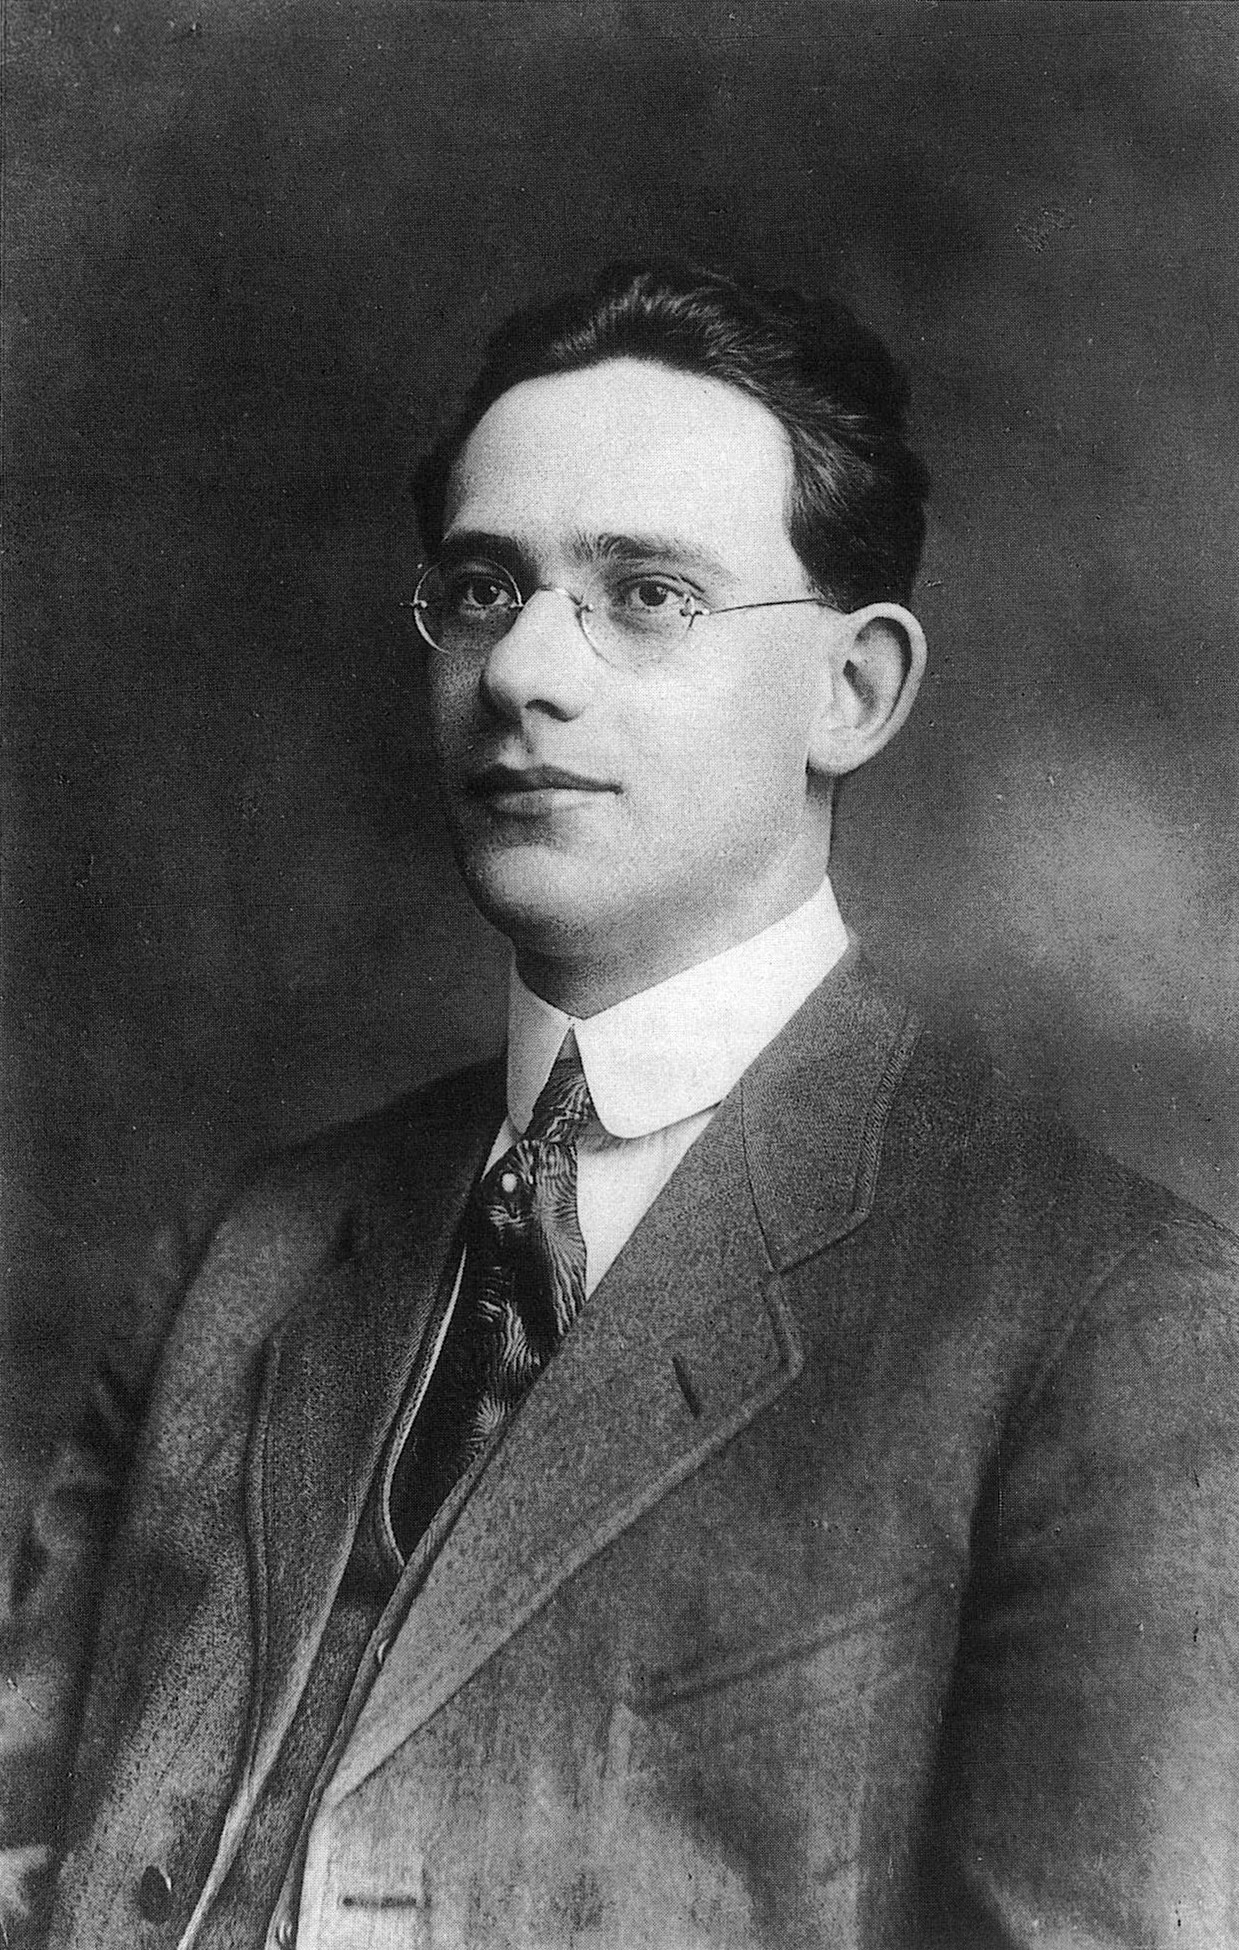
\includegraphics[width=.95\textwidth]{figures/Sapir-1913.jpg}
  \caption{Edward Sapir (1913)}
  \label{fig:ch.sapir.sapir_1913}
\end{wrapfigure}
His \ili{Takelma} grammar (essentially his 1909 dissertation) was
published as \citealt{sapir22:takelma} in volume 2 of the
\textsl{Handbook of American Indian Languages}. This work is truly
incredible in its comprehensiveness and insight when one considers
that it was based on only a month and a half of fieldwork. Around 1917
he wrote his description of \ili{Southern Paiute} (which was only published
some years later, as \citealt{sapir30:s.paiute}); his popular outline
\textsl{Language} \citep{sapir21:language} also appeared during these
years. Together with his monograph on \textsl{Time Perspective}
\citep{sapir16:time.perspective}, these were essentially the only
book-length works {\Sapir} produced in his entire career, but along with
a large number of shorter articles on linguistic and more general
cultural topics, as well as nonlinguistic writings, they make the list
of his publications during his Canadian years impressive
indeed.\footnote{{\Sapir}'s \textsl{Collected Works} on linguistic and
  ethnographic topics are intended to run to a total of 16 very
  substantial volumes, nine of which have appeared as of this date
  (2021).}

While he was in Ottawa, {\Sapir}'s first wife \name{Florence Delson}{Sapir}
suffered a series of mental and physical illnesses from which she
eventually died in 1924. An added disappointment was the fact that his
efforts to develop anthropological research on the native peoples of
Canada were largely halted by the financial and other exigencies of
the First World War. Coupled with his perception of the {contrast}
between the freedom of his student days and the amount of
comparatively unrewarding responsibility incumbent on him as an
administrator, these frustrations increased his feelings of isolation
and alienation.

In this period {\Sapir} began to devote a considerable amount of time to
artistic expression—poetry and music, as well as the writing of quite
a number of (literary) reviews. From 1917 through the early 1930s, he
was a major contributor to \textsl{The Dial} (one of the most
important American literary journals of the time) as well as a
reviewer and writer for other journals such as \textsl{The Freeman},
\textsl{Poetry}, \textsl{The New Republic}, \textsl{The Nation}, and
others far from professional linguistics and \isi{ethnography}. Many of the
same concerns that dominate his nonacademic writing, however, also
appear in connection with his work in \isi{anthropology}. He became
increasingly interested in questions of psychiatry and the nature of
personality, and particularly in the relation between personality and
\isi{culture}.

While his linguistic work always constituted a sort of foundation for
the exploration of such issues, he was generally more interested in
expanding the relation between the study of language and other domains
than in the development of specifically linguistic methodology. As the
field became increasingly self-aware and professionalized in later
years (recall that, in the 1920s, there really was no such distinct
discipline as linguistics at any American university), this would put
his work rather at odds with the tendency of most other linguists to
emphasize the uniqueness of the object of their research and the
methods appropriate to it.

\begin{wrapfigure}{r}{.4\textwidth}
  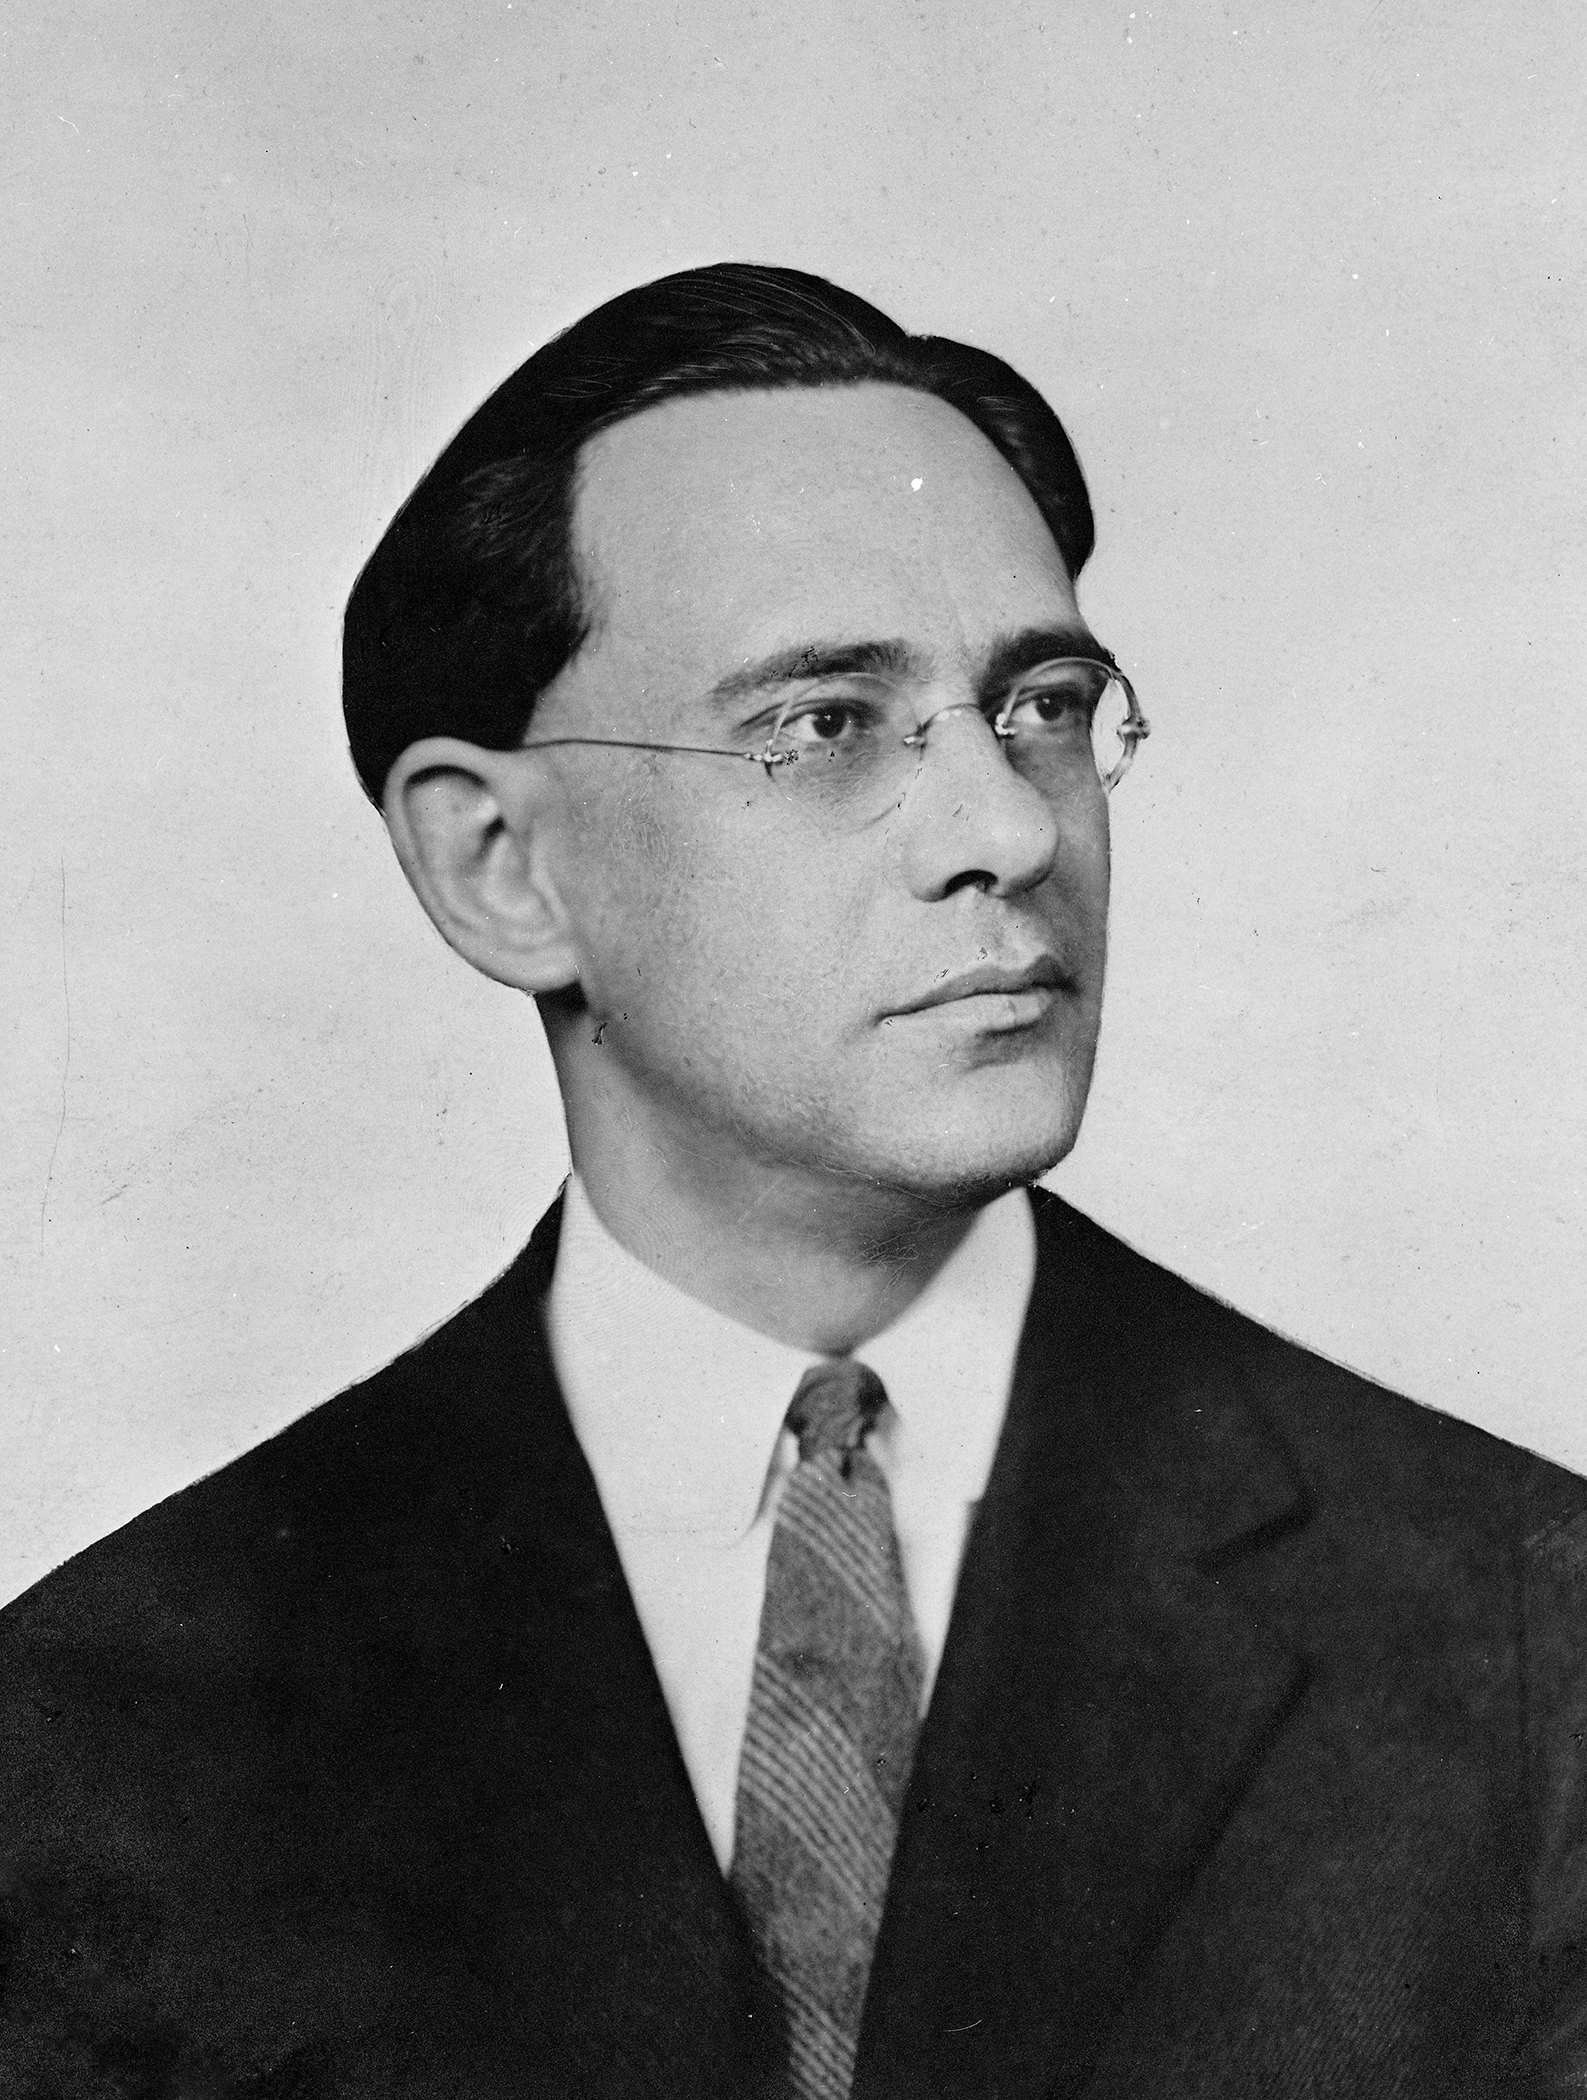
\includegraphics[width=.9\textwidth]{figures/Sapir-1925.jpg}
  \caption{Edward Sapir (1925)}
  \label{fig:ch.sapir.sapir_1925}
\end{wrapfigure}
In 1925 {\Sapir} was offered a position at the University of Chicago,
which he was happy to accept, though he would have preferred a move to
Columbia in New York. At Chicago he had a great many students (many of
whom, with a few exceptions such as {\Hoijer}, later followed him in his
move to Yale); and within a short time he was a major figure in
American \isi{anthropology}. He continued to do fieldwork on several
languages (including \ili{Navajo} and Hupa) and had the opportunity to do
many of the things whose absence he had regretted in Ottawa. In 1926
he was married again, to \name{Jean}{McClenaghan}. For a
time he continued to write poetry (and to participate in the
University of Chicago poetry club); but eventually the pressure of
other work left him little time for anything but his professional
obligations.

Gradually becoming disillusioned with the amount of administrative
effort demanded of him at Chicago, he accepted the very attractive
offer of a Sterling Professorship at Yale in 1931. His appointment
coincided with the establishment of a Department of Linguistics,
although as described by \citet{wells74:lx-at-yale}, this
``Department'' had no budget, or power of appointment, or
undergraduate program, or even a Chairman (the central administrative
figure being the Director of Graduate Studies). It was, rather, a PhD
program and a grouping of courses offered by faculty who all held
appointments in some other Department.  Linguistics at Yale did not
become a real (i.e., budgetary) department until 1959: in {\Sapir}'s
time, it was what would today be called an inter-departmental degree
program.

{\Sapir}'s appointment as Chair of Anthropology, itself a program within
a larger Department of Social Sciences, made him Sterling Professor of
Anthropology and Linguistics. As \citet{haas84:sapir.training} recalls
the situation, he encouraged his students in Anthropology working on
unwritten (or ``primitive'') languages to take courses in Linguistics
that would prepare them for comparative and historical studies as well
as synchronic description.

\begin{wrapfigure}{r}{.4\textwidth}
  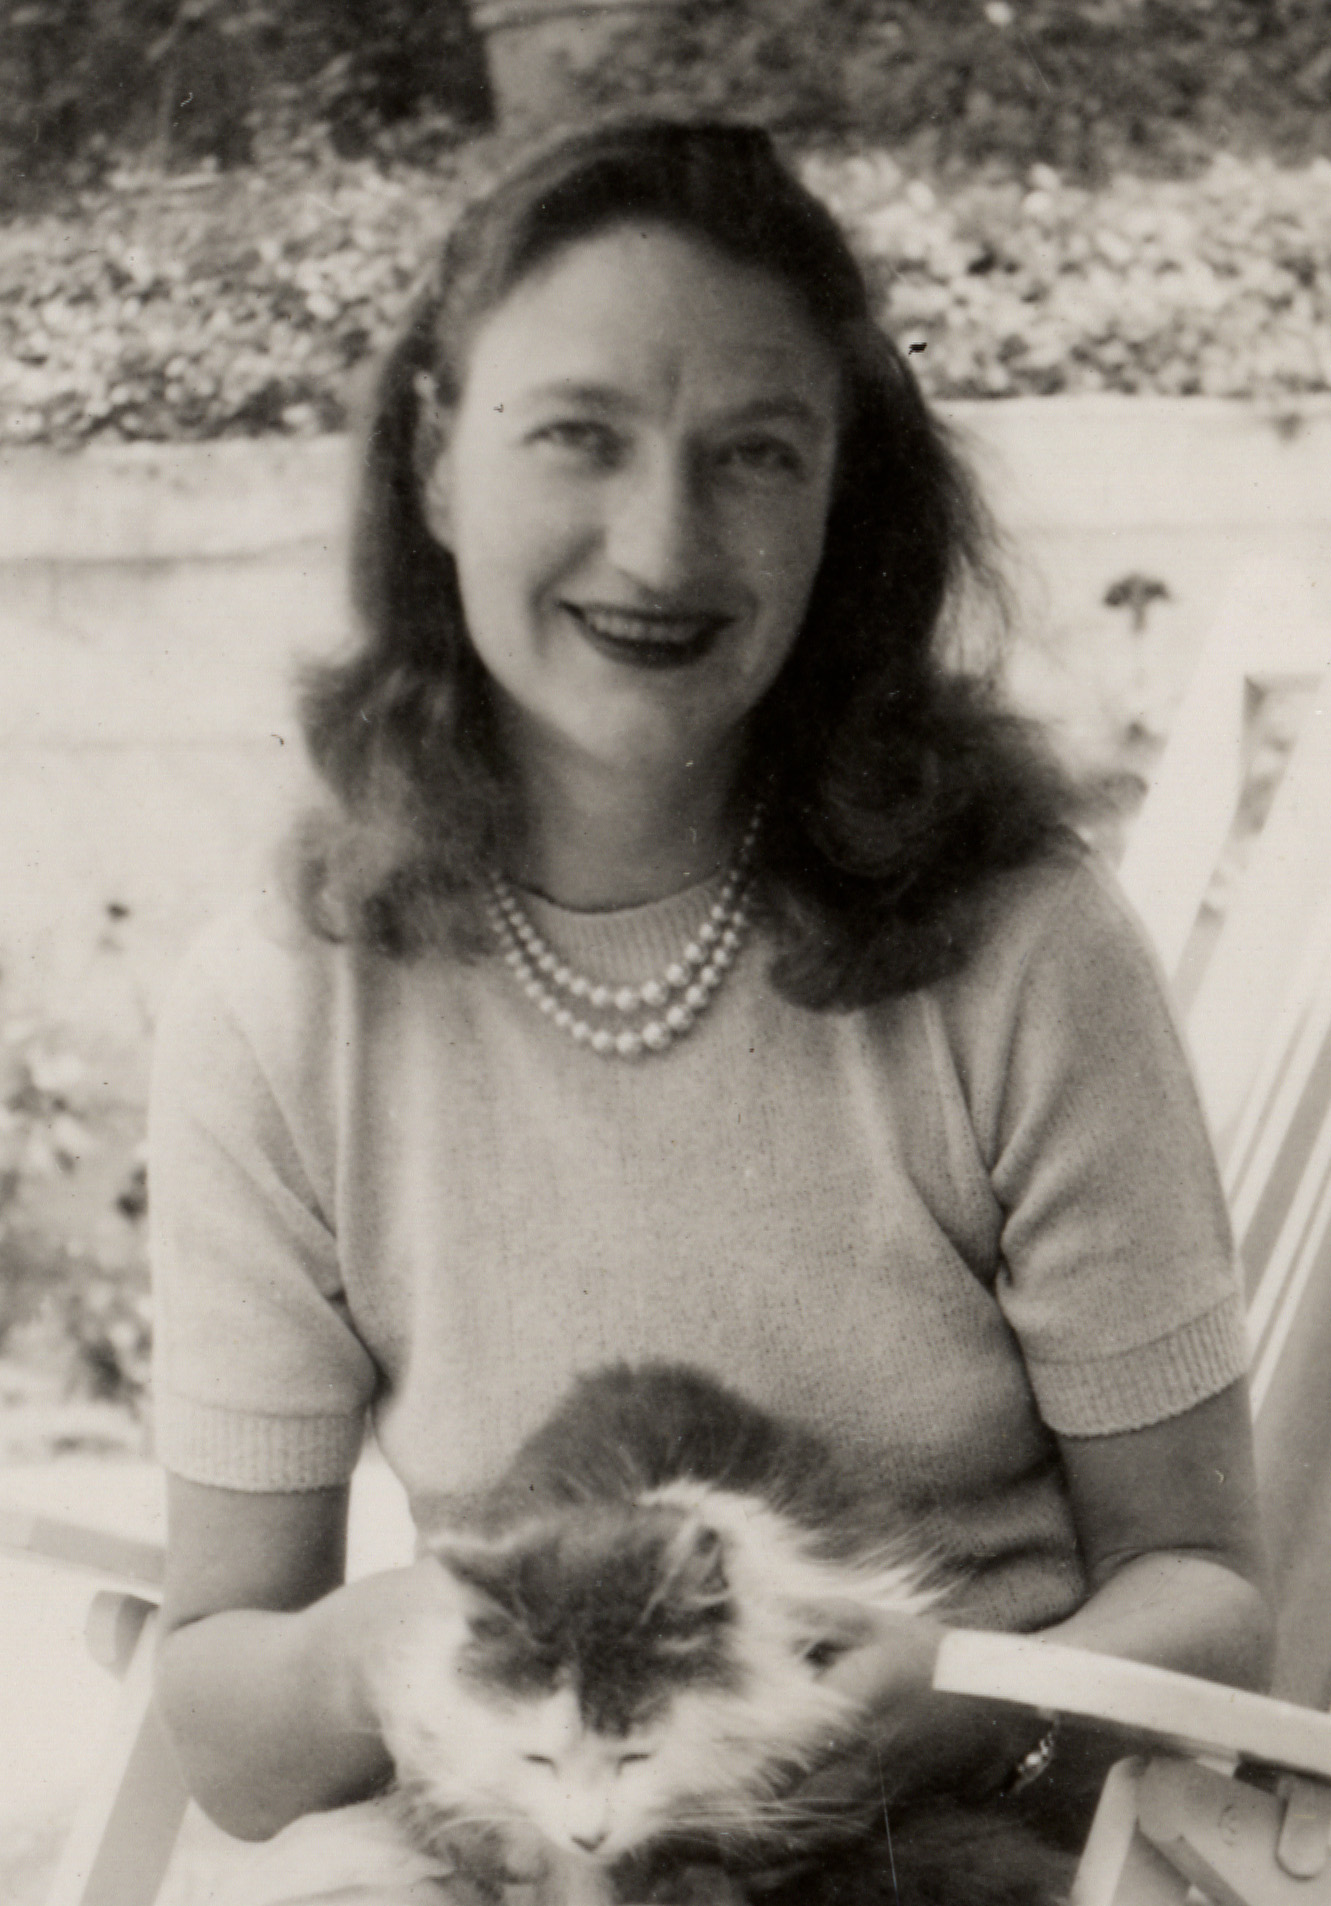
\includegraphics[width=.9\textwidth]{figures/MaryHaas_cat.jpg}
  \caption{Mary Haas and cat}
  \label{fig:ch.sapir.haas_cat}
\end{wrapfigure}
Sapir\ia{Sapir, Edward}'s offer from Yale included funding to allow three of his
students---\name{Stanley}{Newman}, \name{Walter}{Dyk} and \name{Morris}{Swadesh}---to come
with him. {\Swadesh} and Mary {\Haas} had been married in the spring of 1931
(spending their honeymoon doing fieldwork on ``Nootka'' (Nuuchahnulth)
and ``Nitinat'' (Ditidaht) on Vancouver Island), and {\Haas} came with
{\Swadesh} without separate support. He also attracted \name{Carl}{Voegelin} (a
student of {\Kroeber}'s), \name{Benjamin}{Whorf} (a non-student who sat in on his
classes) and a number of others, though very few beginning students,
in {contrast} to his years at Chicago.

Haas\ia{Haas, Mary Rosamond} and {\Swadesh} were divorced in 1937 
(by mutual agreement, according
to \citet{heaton.etal21:women.in.lx}, on the basis that {\Haas}'s job
propects would be much better if she were unmarried). She had
completed her dissertation on Tunica in 1935 (an abridged version of
which eventually appeared as \citealt{haas41:tunica}, the only part of
a projected volume 4 of the \textsl{Handbook of American Indian
  Languages} that was ever published), but especially in Depression
times, her job prospects were poor. {\Sapir} helped her find support at
Yale for a few years, but the sexist nature of academia had its
effects:
\begin{quotation}
  In a formal letter to A. L. {\Kroeber}, dated June 17, 1935 (Bancroft
  Library, UC Berkeley), {\Sapir} recommended {\Swadesh} (`there is no
  better linguist in the country') for a research position or
  instructorship at Berkeley, adding: `Mrs. Swadesh has just obtained
  her Ph.D. with an excellent thesis on Tunica [and] at no extra cost
  to your department, or at very little extra cost, you would be
  getting the benefit of another linguist.' He followed this up with a
  personal letter, dated July 24, 1935 (Bancroft Library, UC
  Berkeley), in which he wrote: `{\Swadesh} and his wife are \ldots\
  likely for an indefinite period---perhaps the rest of their
  lives---to be committed to specialist work in American Indian
  linguistics \ldots\ the Swadeshes love languages as you love
  decorative art and chess. Their combined energy is enormous and a
  very little effort to fund them would be richly rewarded.' Two years
  later, {\Sapir} once again recommended {\Haas} to {\Kroeber} for a position
  at Berkeley, this time independently of {\Swadesh}: `I do not know much
  of what your plans are for a geographic survey of American Indian
  linguistics in general or California linguistics in particular, but
  if you have such a scheme in mind, I should think that Mary {\Haas}
  would be a particularly good bet. My respect for her work has grown
  steadily from year to year. She is not as brilliant as Morris but
  more interested in historic problems and fully as accurate in her
  field methodology' ({\Sapir} to {\Kroeber} August 5, 1937, Bancroft
  Library, UC Berkeley). {\Haas} once told Golla\ia{Golla, Victor} that she knew of these
  letters, but was neither surprised nor offended by the blatancy of
  {\Sapir}'s male chauvinism (`no extra cost', `not as brilliant'). The
  reality of academic life in the 1930s, she explained, was that men
  were always given preference, and {\Sapir} knew that it was easier to
  sell {\Swadesh} than herself to a figure like {\Kroeber}.\\
  \citep[827, fn. 2]{golla.matisoff97:haas.obit}
\end{quotation}

\begin{wrapfigure}{r}{.35\textwidth}
  
\includegraphics[width=.9\textwidth]{figures/morris-swadesh_army.jpg}
  \caption{Morris Swadesh}
  \label{fig:ch.sapir.swadesh_army}
\end{wrapfigure}
Swadesh\ia{Swadesh, Morris} taught briefly at the University of Wisconsin, but his
outspoken political views got him fired in 1939, and he moved to
Mexico.  During World War II he participated in the Army Intensive
Language Program, and after the war was hired at the City College of
New York. His politics got him caught up in the Red Scare of the late
1940s, and he was again fired. He returned to Mexico, where he
continued to teach linguistics until moving to The University of
Alberta in 1966, where he died in 1967.

In New Haven, {\Sapir} encountered a considerable degree of anti-semitic
feeling. Unusually, his appointment at Yale was to the Graduate School
only, and not, as in most cases, also to Yale College, it not being
considered suitable for Yale undergraduates to be taught by a Jew, and
in any case there was no undergraduate program in Linguistics. He was
also apparently blackballed from the Yale Graduate club, the
institution where most serious academic business among the faculty was
transacted. In reaction to this, the Linguistics faculty withdrew
\emph{en masse} from participation in the Graduate Club, and
henceforth met at a \emph{Stammtisch} in the University Commons dining
hall.\footnote{\name{Stanley}{Insler}, personal communication.}  He was still
by no means free of administrative obligations, and complained that he
had no time to himself for research. In 1937-38, these irritations
were exacerbated by a series of heart attacks, and he died of heart
disease in 1939.

{\Sapir}'s background as a student of {\Boas} obviously had a significant
influence on his later views. His first work (such as his \ili{Takelma}
grammar) is clearly within that tradition, though it also shows
considerable originality and independence---enough so that {\Boas} had
not thought it suitable for inclusion in the first volume of the
\textsl{Handbook}. In fact, more of {\Sapir}'s apparently distinctive
position can be traced to its Boasian roots than is sometimes
recognized: the {stress} he put on the psychological foundations of
linguistic knowledge, the extent to which a language can be studied in
order to analyze the unconscious categorization that underlies the
worldview of its speakers—these basic goals are a direct working out
of {\Boas}'s view of language as ``a window on the soul.''  {\Sapir}'s
original contributions to the development of a comprehensive
theoretical view of language and its structure are not in any way to
be minimized, but it should also be recognized that both in general
and in many of its specifics, the resulting systematization has a
great deal in common with the position sketched (and to some extent
practiced) by {\Boas}. The influence of his study of \name{Johann}{Herder} for
his Master's thesis may also have played a role in the development of
his thinking.

Such an approach to language as a profoundly internal mental
phenomenon must be contrasted (as of course it usually is) with the
behaviorist, positivist, and mechanist climate of research which grew
up in the sciences generally during the 1930s and 1940s. The central
figure in the rise of such an approach to linguistics was Leonard
{\Bloomfield}, whose work will be the subject of the following
chapter. Typically, presentations of the history of American
linguistics associate {\Sapir}'s views with the 1920s and early 1930s,
and treat {\Bloomfield} as succeeding {\Sapir}. As stressed by
\citet{hymes.fought81:structuralism} and
\citet{murray93:theory.groups}, however, the actual chronology is
somewhat more complicated.

In fact, {\Bloomfield} and {\Sapir} were essentially contemporaries; and if
{\Sapir} was clearly a prominent figure in \isi{anthropology} in the 1920s
before {\Bloomfield} became well known, the 1930s were a time in which
both were active and influential. Certainly {\Sapir} was more prominent
in the relations between American and European linguists in the
development of phonology; he corresponded extensively with {\Trubetzkoy}
in the early 1930s (though these letters were destroyed before his
death, and cannot now be examined), and the latter spoke positively of
him on many occasions. When the \isi{International Phonological Association}
was established under the influence of the Prague school linguists in
1932, it was {\Sapir} who was elected as the sole American member of its
board, and he continued to be the primary link between European and
American phonologists until his death.

{\Sapir} and {\Bloomfield} of course knew and interacted with one another to
a considerable extent (they were colleagues at Chicago, and in part in
competition for students there between 1927 and 1931), though it seems
that while their relations were perfectly cordial, they were anything
but fast friends. {\Sapir}'s own style of research was based much more on
brilliance and intuition, searching for dramatic insights whose
foundation might (or might not) be confirmed by later systematic
investigation. {\Bloomfield} was much more methodical in the way he felt
theoretical propositions ought to be worked out, and while admiring
{\Sapir}'s more virtuosic approach, he referred to him (at least in
matters outside of language) as a ``medicine man'' (\name{Carl}{Voegelin}, as
quoted in \citealt[540]{hockett70:bloomfield.anthology}).  {\Sapir}, for
his part, ``admired {\Bloomfield}'s ability patiently to excerpt data and
to file and collate slips until the patterns of the language emerged,
but spoke deprecatingly of {\Bloomfield}'s sophomoric psychology''
(\emph{Ibid}., pp. 539-40). Such a {contrast} in styles cannot have made
for an easy cooperation; nor were their relations improved, one
imagines, by the fact that some of the best students at Chicago left
to follow {\Sapir} to Yale in 1931. Overall, if one had to bet in the
early 1930s on the likely outcome of the inevitable rivalry between
the two, one would surely have had to predict the continued ascendancy
of {\Sapir}.

While {\Sapir} did indeed continue to exert an important influence on
linguistics throughout the 1930s, 1940s and 1950s through his own work
and that of a series of students (and their students in turn), his was
increasingly a peripheral, even eccentric position in relation to the
main stream of development of the field. {\Sapir} was thus gradually
eclipsed by {\Bloomfield}, for a number of rather superficial (but
nonetheless important) reasons.

Among these is surely the fact that {\Sapir} died in 1939 and was thus
unable to exercise the influence of his undeniably attractive
abilities in the years during and right after World War II. Further,
his students and closest associates were, after the war, either dead
({\Whorf}), unemployed (and subject to political persecution, in the case
of {\Swadesh}), or employed in universities on the West Coast ({\Haas},
{\Hoijer}, {\Newman}) where their influence on academic politics was almost
negligible. In addition to these factors, there was the fact that
{\Bloomfield} had written a major textbook \citep{bloomfield:lg} which had a
formative influence on virtually all the immediately following
generations of students in linguistics, while {\Sapir} had not; and also
the fact that {\Sapir} taught only once at the (summer) Linguistic
Institute (a major institution in the formation and training of a new
generation of scholars who saw themselves professionally as
linguists), while {\Bloomfield} taught there several times.

Finally, one must not neglect the fact that {\Bloomfield}'s appeal to a
positivist, mechanist philosophy of science was completely in tune
with the `ideological' climate of academic research at the time. If
linguists saw a major part of their task as the establishment of a
distinct discipline of linguistics which was not simply a part of
Germanics, Romance, Semitics, comparative philology, \isi{anthropology},
etc., it seemed that the way to achieve this goal was by stressing the
status of linguistics as a science; and here {\Bloomfield}'s approach
seemed much more appropriate than {\Sapir}'s \isi{mentalism} and flashes of
intuition. The appeal of research which takes on at least the
trappings of `science' has of course not disappeared; one can argue
about the extent to which such considerations distort scholarly
judgments in particular cases, but there is no question that they
contributed to the relegation of the `{\Sapir} school' to a marginal
position in American linguistics in the late 1930s and subsequently.

\section{Sapir's view of the nature of language}

It is on the basis of his conception of the object of study in
linguistics that {\Sapir} differs most fundamentally from the approach to
language which arose during the 1930s and came to dominate research in
America, especially after World War II. In {contrast} to these later
developments, {\Sapir} believed in the importance of a rich and highly
structured domain of interior mental phenomena, including in
particular virtually all of what is essential to the nature of
language. In chapters~\ref{ch.bloomfield} and~\ref{ch.structuralists},
we will trace the development by which, for many linguists, language
came to be considered as exhaustively studiable in terms of its
external manifestations: sounds, and patterns of observable behavior
to which `\isi{meaning}' could be reduced (at least programmatically, in
principle). For {\Sapir}, in {contrast}, these physical aspects of language
were merely peripheral (almost incidental) concomitants of a reality
which is to be sought in the mind, and whose study provides invaluable
information about the nature and structure of human cognitive
activity.

The consequences of this difference are quite clear in the domain of
interest to us here, the study of phonology. For nearly all
theoreticians of the time, certainly including {\Sapir}, a central role
is played in phonological structure by a basic segment-like element:
the \emph{phoneme}. Linguists who approached language strictly in
terms of its external manifestations, however, founded this notion on
the study of the physical sounds of speech: through extracting the
acoustic or auditory properties which distinguish one \isi{speech sound}
from another, or through an analysis of the distribution of various
physical segment types. {\Sapir}'s conception is quite different, since
the physical implementation of a \isi{phoneme} is among its least
interesting properties. True, phonemes are realized in the sounds of
speech; but their essence is rather something in the mind whose most
important features may be unrelated (or even in direct contradiction)
to measurable aspects of a physical event. In a much-quoted passage,
the central reality of \isi{sound structure} is likened to ``an ideal flow of
phonetic elements [\ldots] heard, inadequately from a purely objective
standpoint, as the intention of the actual rumble of speech''
\citep[56]{sapir21:language}.

The claim that language is primarily a psychological rather than a
physical activity does not at all imply that the structure of this
activity is given in advance by the innate, biologically controlled
organization of the human brain. On the contrary, {\Sapir} stresses in
the introductory chapters of \textsl{Language} his view that ``speech
is a human activity that varies without assignable limit as we pass
from social group to social group, because it is a purely historical
heritage of the group, the product of long continued social usage.'' He
specifically contrasts walking, which ``is an organic, an instinctive
function (not, of course, itself an instinct)'' with speech, which ``is
a non-instinctive, acquired, `cultural' function''
\citep[4]{sapir21:language}. Language, like the rest of \isi{culture}, is
something that we learn more or less as we find it, and because it is
there, rather than because we are in some way inherently predisposed
to acquire a system of a particular nature.

{\Sapir}'s {stress} on the cultural (rather than biological) basis of
language can be traced rather directly to the views of {\Boas}. In
American \isi{anthropology} in the twentieth century, this {stress} on the
social environment rather than biological background as the source of
cultural institutions affects many more domains of study than just
language; and {\Boas} is often cited as the dominant figure championing
such a position in anthropological studies as a whole. His student
\name{Margaret}{Mead}, for example, is generally felt to have been urging a
fundamentally Boasian view in her enormously important study of {Samoan}
society (\citealt{mead28:samoa}, to which {\Boas} wrote a foreword),
which argued for a cultural rather than biological foundation for many
human attitudes (aggressivity, jealousy, the turmoil of adolescence,
etc.).

In the social and political context of the 1920s and 1930s (and
subsequently), this {stress} on environment rather than heredity as a
determinant of human cognitive functions and attitudes was generally
felt to be an important contribution of the social sciences, useful in
supporting `liberal' positions on desirable social {change}. Subsequent
controversy about Mead\ia{Mead, Margaret}'s work, initiated by
\posscitet{freeman83:mead.samoa} attack on her account of life in
Samoa, has centered on the claim that she misrepresented (or at least
mis-perceived) the facts of {Samoan} society in order to exaggerate the
importance of such social factors at the expense of inherited ones—a
predisposition she is presumed to have acquired from {\Boas}.

{\Boas}'s {stress} on diversity (as opposed to some sort of biologically
inherited uniformity) played an essential role in forcing the
recognition that languages (or cultures) very different from those of
Europe had to be approached in their own terms, rather than as
imperfect or primitive approaches to some uniform ideal
system. Obviously, this position has general cultural and political
implications for many issues beyond the narrow question of how a
particular science (linguistics or \isi{anthropology}) should be
organized.

In urging a non-biological view of the essential nature of language,
{\Sapir} was supporting the same point in what seemed the most logically
straightforward way; for if human language is actually determined in
its structure by innate, biologically inherited factors, it would
appear that it should present a more or less uniform organization (at
least within a genetically uniform sampling of humanity). The observed
diversity of human languages and their historical evolution, however,
seems to contradict this view rather directly. Based as they were on a
strict `organic' determinism, the typologies of language and its
evolution that were proposed in the nineteenth century could be shown
to be hopelessly inadequate as a characterization of linguistic
reality: a result which {\Sapir} felt was not at all an accident but a
direct consequence of their inadequate underlying conception of the
nature of language.

A number of factors thus led {\Sapir} to {stress} the social as opposed to
biological basis of linguistic structure: his education with {\Boas}, the
developing climate of opinion in academic \isi{anthropology} in the 1920s
and 1930s in conjunction with liberal political views during the same
period, and the apparent necessity to make such an assumption in order
to explain the evident diversity of human languages and their failure
to follow the same evolutionary sequence. In seeing the structure of
language as strictly an accidental consequence of cultural
environment, however, free of any sort of biologically grounded
necessity, this view leads logically to a major problem for
linguistics. In the passage quoted above, language is argued to be ``a
human activity that varies without assignable limit''; but this implies
that there are absolutely no (non-accidental) \isi{universals} of linguistic
structure—a finding at variance with the manifest fact that, if
languages may be very different from one another in many ways, we
still have no difficulty at all in knowing what sort of activity and
system in a society to call `language', and in fact no difficulty in
finding many ways in which languages resemble one another.

{\Sapir} was of course well aware of the fact that languages do not
actually differ from one another in absolutely arbitrary ways, and
that there are at least some generalizations that are valid across
languages. Identifying specific dimensions along which languages may
in fact differ from one another (and thus by implication, properties
in terms of which they are comparable), through the development of an
explicit typological scheme applicable in principle to any language,
occupied a considerable amount of his efforts. To be coherent, the
position that any comprehensive \isi{typology} is possible must rest on the
assumption that there are some \isi{universals} of human language; and once
he asserted that these do not have basis in our biological nature as
\emph{Homo sapiens}, it was logically incumbent on {\Sapir} either to
propose some other foundation for them or to deny their existence.

The denial that there are any significant linguistic \isi{universals} was
the path often taken by American structuralists (see
\posscitet[96]{joos57:readings} famous statement about the arbitrary
differences possible among languages, cited in the previous chapter),
but not the view of {\Sapir}: ``It would be too easy to relieve ourselves of the
burden of constructive thinking and to take the standpoint that each
language has its unique history, therefore its unique structure. Such
a standpoint expresses only a half truth''
\citep[121]{sapir21:language}. In fact, we observe that languages show
similarities in structure despite being unrelated to one another (at
least in the time frame relevant to the development of the features in
question). He suggests that these similarities may have their origin
in the fact that ``a language changes not only gradually but
consistently, that it moves unconsciously from one type towards
another, and that analogous trends are observable in remote quarters
of the globe'' (\emph{Ibid}); but, whatever their source, it is
important for the linguist to develop a framework in which both the
similarities and the differences among languages can be adequately
represented. This he attempts to do in chapter 6 of \textsl{Language}.

He observes first of all that previous classificatory schemes were
much too limited to encompass the actual variety of human
language. There are several reasons for this: they usually involved
too few categories (e.g., `isolating' vs. `agglutinating'
vs. `inflecting'); they were established with regard to only a single
aspect of linguistic structure (typically the formal \isi{mechanism} of word
formation); they were based on a sample of too few languages; and
(most importantly), they were guided by the aim of arriving at a
uniform evolutionary sequence culminating in some particular
type—often the language of the investigator, or perhaps classical
\ili{Greek} and \ili{Latin}—as the manifestation of the ultimate stage of the
evolution of civilized expression.

{\Sapir}'s own scheme is certainly more ramified than any other proposed
up to the time. It would take us much too far afield here to explore
it in detail (see \citealt{sra90:krems} for some discussion), but we
can note that it is based on three quite different dimensions. One of
these (the most innovative aspect of his framework) is the type of
concepts expressed in a given language. He assumes that every language
must express a range of basic (concrete) concepts corresponding to the
reference of simple lexical items, especially nouns and verbs. In
addition, every language must express a certain range of pure
relational concepts, which ``serve to relate the concrete elements of
the proposition to each other, thus giving it definite syntactic
form.'' The positing of such categories as necessary ones is already a
significant departure from the strong view that languages are in
principle arbitrarily different from one another.

In addition to these minimal requirements, corresponding essentially
to lexical roots in the one case and to purely syntactic inflectional
categories in the other, languages may allow for two sorts of
interpenetration of referential and relational constructs. As one
possibility, languages may express \emph{derivational} concepts, by
which the meanings of radical items are modified to form new lexical
items (e.g., an agentive operator which takes basic concrete verbs and
produces nouns with the sense `one who typically or often [verb]s');
and as another, they may allow for certain \emph{concrete relational}
categories. The latter are categories such as agreement in person, or
in `natural' (as opposed to purely arbitrary) gender: categories that
play a role in inflection and the organization of syntactic structure,
but which nonetheless have a sort of semantic or referential basis as
well. He arrives at four general categories of language, depending on
whether one, the other, both, or neither of these possibilities is
realized in a given language. It can be seen that {\Sapir} assumes a
division between \isi{syntax} and \isi{lexicon} as the basis for a distinction
between inflectional and derivational morphology.  That such a point
of view furnishes the only satisfactory foundation for this
traditional opposition is argued in generative terms by
\citet{sra82:wheresmorphology}.

{\Sapir}'s second dimension of linguistic \isi{contrast} is the traditional one
of the formal means by which those concepts which find expression in a
given language are realized: isolating (where each \isi{concept} is
expressed in a separate word), agglutinating (where distinct concepts
are expressed by distinct, nonoverlapping parts of words), fusional
(where some amalgamation of distinct concepts into single or
\isi{overlapping} parts of a word is found), and symbolic (where some
concepts are expressed not by a separable part of the word, but rather
by the structural relation between one word and another, as in cases
of Ablaut like
\emph{sing}/\emph{sang}/\emph{sung}/\emph{song}). Employing such a
classification in addition to that distinguishing types of \isi{concept}
allows {\Sapir} to characterize a language in which concepts of one type
(e.g. derivational ones) are expressed in one way (e.g. symbolically),
while those of another (perhaps pure relational ones) are expressed in
another (e.g. by agglutinating affixes). 

Finally, {\Sapir} allows for the
classification of languages along a third dimension, that of ``degree
of synthesis'' or typical conceptual complexity of individual words—an
essentially continuous scale ranging from \emph{analytic} through
\emph{synthetic} to the extreme of \emph{polysynthetic}.

{\Sapir}'s overall classificatory framework is much more complex, and
accordingly more delicate than any of the traditional
nineteenth-century schemes. One may still question whether it provides
dimensions that are adequate to characterize the significant
differences and similarities among the world's languages; but that is
not our purpose here. Rather, what is interesting is the role which
{\Sapir} thought a \isi{typology} plays in a theory of language. Precisely
because it provides a number of potentially independent dimensions,
rather than a single unidirectional scale like most of those that
preceded it, it serves a fundamentally synchronic, descriptive
purpose. It is intended, that is, to describe what the structure of a
language is, rather than how far along a presumed evolutionary scale
it has progressed.

It is reasonably clear also that a primary goal of typological
research today is not intended to be served by {\Sapir}'s
framework. Current typological work (at its best, at least) seeks to
establish necessary connections among phenomena: for example,
Greenberg's celebrated \isi{typology} of SOV, SVO, and VSO languages was
intended not simply to specify the range of freedom available to the
languages of the world with respect to the major constituents of the
sentence, but also to bring out connections between that relative
order and other features, such as the relative order of nouns and
modifying adjectives, the choice of prepositions or postpositions,
etc. Precisely because {\Sapir}'s schema provides nothing beyond a range
of mutually independent categories, it lacks such a logical structure,
and in fact there is little evidence {\Sapir} looked for implicational
relationships among typological parameters provided by his system.

On the other hand, {\Sapir} did think there were profound relationships
which might eventually be discovered between the categories of
linguistic structure in his terms and basic aspects of \isi{culture} and of
mental life. Together with \name{Benjamin Lee}{Whorf}, he was largely responsible
for bringing to prominence in anthropological discussion the claim
that the structure of our language determines many aspects of the way
in which we see and structure the world. In other words, the
categorizations imposed by language channel and structure our thought,
leading us to see some connections among phenomena while ignoring
others—differing connections for the speakers of differing
languages.

This is of course a natural development of {\Boas}'s ideas about the
importance of differences in the categories languages treat as
obligatory, optional, or unexpressed; but {\Sapir} and {\Whorf} pursued the
psychological implications of this position much further than
{\Boas}. While he did not claim to be able to demonstrate actual
connections between the categories of his \isi{typology} and
language-specific cognitive differences, {\Sapir} did feel that the
elucidation of such connections was a role \isi{typology} should be able to
play.

I should also mention two other potential applications of a
typological schema according to {\Sapir}, both in the sphere of
historical linguistics. First, there is his celebrated theory of
linguistic ``\isi{drift}.'' This notion is intended to represent the fact
that, even after a language has divided into a number of distinct,
separated speech communities, the evolution of the several individual
descendants of that language may well continue to pursue very similar
lines. This leads to a state in which multiple members of a family
make the same innovation quite independently of one another (or at
least without any necessary contact between them)—which of course
makes the historical linguist's task that much harder in determining
which features of the daughter languages should be attributed to their
common ancestor. Often presented as something quite mystical, the most
straightforward way to interpret {\Sapir}'s notion of linguistic \isi{drift} is
simply as the claim that change is motivated by structural factors,
and that such structural factors, present in the ancestor of a group
of related languages, may persist and continue to influence their
later evolution even after their separation. Ideally, a \isi{typology} ought
to provide categories in terms of which to identify such structural
factors and clarify their influence on change.

Additionally, \isi{typology} played a role in {\Sapir}'s own concrete
historical work. He did extensive research of this sort, including
historical studies in \ili{Indo-Europe\-an} (especially Tocharian) and
\ili{Semitic}, but especially in the classification of American Indian
languages. One of his best-known theoretical claims, in fact, was his
far-reaching proposal for a genetic classification of the languages of
North and Central America into six large groups. This classification
was based on a large number of rather remote linguistic relationships,
many of which could not be proved or even significantly supported by
standard comparative evidence; and one naturally asks what {\Sapir} based
his assertions on.

It is fairly clear that most of those claimed genetic connections
which {\Sapir} posited without support from common vocabulary rested on
presumed similarities in structure—just the sort of parallels that a
typological framework ought to be able to make explicit. The
evidential role of such structural similarities is particularly strong
within {\Sapir}'s general perspective on language as culturally based,
but otherwise largely arbitrary; if the role of factors other than
cultural transmission in determining the structure of a language is
comparatively small, it should follow that structural similarity is
strong presumptive evidence of a genetic relationship, since the
preservation of such factors over the period of evolution from a
common ancestor is virtually the only (nonaccidental) \isi{explanation} for
their presence. The role of \isi{typology} here is to provide an instrument
sensitive enough to identify such similarities; once identified, such
a \emph{prima facie} case for genetic unity must eventually be
supported by standard comparative evidence, but \isi{typology} ought to show
the historical linguist where to begin looking.

If I have devoted so much space to a consideration of {\Sapir}'s views
on \isi{typology}, it is not because of the interest his specific proposals
hold for the modern reader. Rather, it seems important to understand
the central role which the general notion of a typological
characterization of linguistic structure played in {\Sapir}'s view of a
theory of language. An understanding of that role, in turn, makes
clearer the sense in which {\Sapir} construed language as a psychological
phenomenon. As an aspect of human mental and cognitive life rather
than merely an external system of interpersonal signals, language
plays a profound role in determining the way we see and organize the
world, but its own structure is in turn determined culturally, in an
external and contingent fashion that allows little or no role for
innate or other biological factors. For {\Sapir}, the fundamental problem
of linguistics was thus not the construction of a `theory of grammar'
but the elucidation of the relationship between language on one hand
and \isi{culture} and personality on the other.

\section{Sapir's conception of phonological structure}

\begin{wrapfigure}{r}{.3\textwidth}
  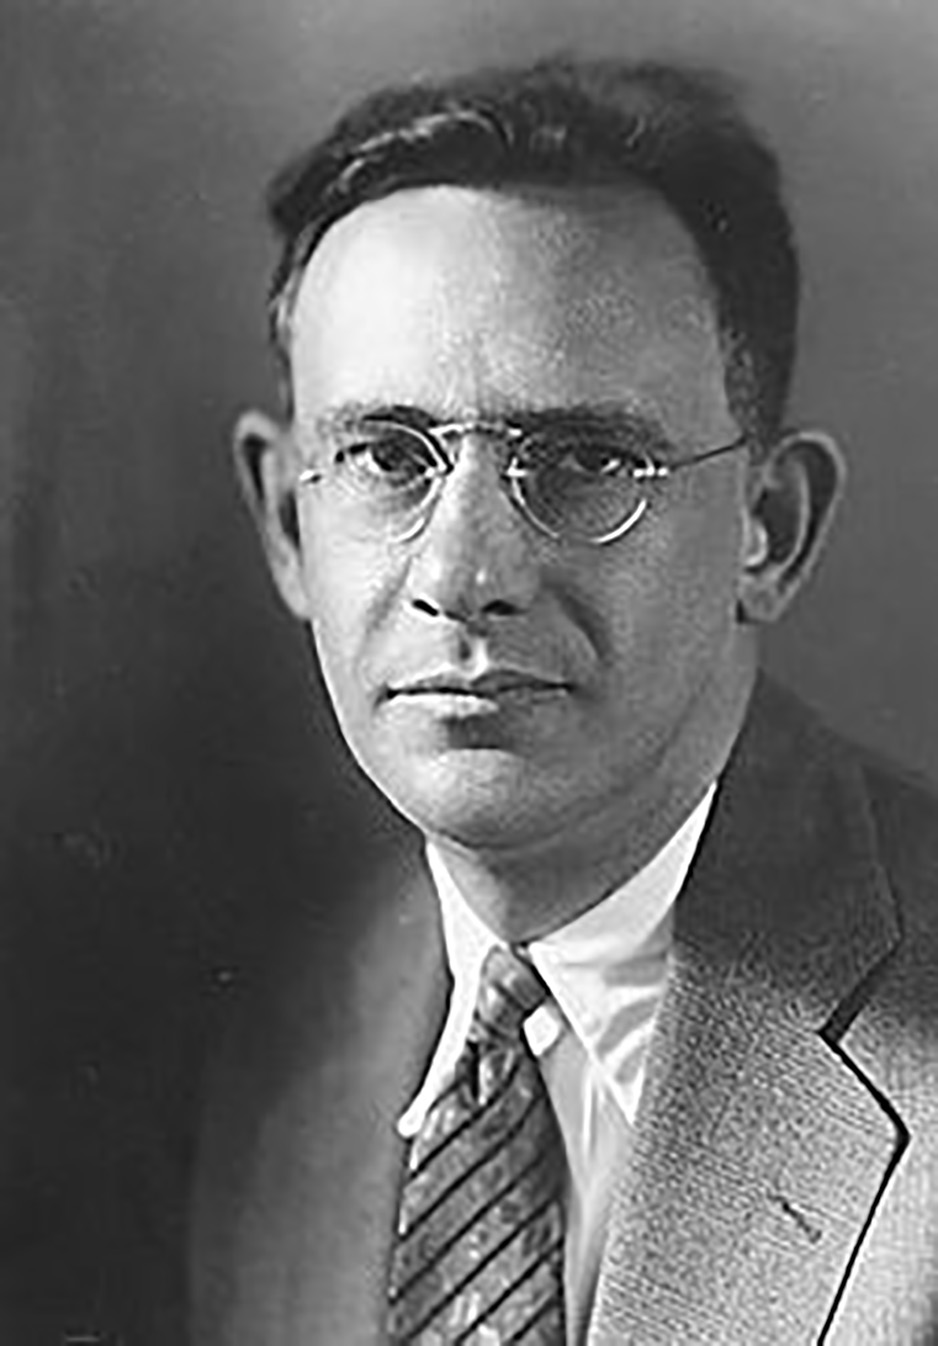
\includegraphics[width=.95\textwidth]{figures/Sapir_0.jpg}
  \caption{Edward Sapir (ca. 1930)}
  \label{fig:ch.sapir.sapir_stock}
\end{wrapfigure}
In discussing the role of sounds in language, {\Sapir} starts from a
perspicuous comparison of an articulatory gesture as it functions
linguistically, and what is effectively the same gesture as it might
be used nonlinguistically. Though physically identical in all relevant
respects, these differ dramatically in their integration with other
similar gestures, both syntagmatically and paradigmatically—i.e., both
in terms of their place in a sequence of human activities, and in
their relation to other, alternative gestures. They also differ in
what counts as an accurate {performance} of the gesture in question,
but, most importantly, they differ in the intention underlying the
gesture in question. Non-speech gestures have directly functional
significance, while the same gestures when used linguistically serve
simply as a ``link in the construction of a symbol.'' This sort of
distinction between a physical act and its linguistic uses is
reminiscent of {\Saussure}, but it should be noted (apart from the fact
that {\Sapir} hardly ever refers to other scholars at all) that {\Sapir}
never refers to {\Saussure} in his theoretical writing and it is quite
unlikely that the \textsl{Cours} would have made it to Canada during
World War I or its immediate aftermath.

It follows, then, that the essential nature of a sound as used in
speech lies in this special character of the intentionality underlying
it: in the fact of what a speaker has in mind in producing it, not the
physical details of the production itself. {\Sapir} draws a useful
{analogy} between sounds in speech and other tools used by humans: a
club is a club not because it has a particular physical form but
because it is put to a particular use. Phenomenological philosophers
such as Heidegger\ia{Heidegger, Martin} make a similar point in arguing that the logically
prior reality of a tool such as a hammer is its ``readiness to hand''
(i.e., its suitability for fulfilling particular intentions of a
conscious user), and that its ``presence at hand'' (i.e., its specific
character as a physical object with certain dimensions, weight, etc.)
is an aspect that arises only secondarily, when we step back from its
basic being as a hammer to regard it as a mere object.

The fundamental nature of a \isi{speech sound} is thus to be sought in the
uses to which it is put in the intentions of a speaker. This reality
is a mental rather than a physical one, and it is exactly this
`\isi{mentalism}' that is generally taken to characterize {\Sapir}'s view. To
say that the basic unit of \isi{sound structure} (the \isi{phoneme}) has a
psychological basis, however, is to tell only part of the story. Even
if the physical properties by which the speaker's phonemic intention
is realized are logically secondary from a linguistic point of view,
that does not mean they are unreal, irrelevant, or completely
arbitrary. Even if ``a club is not defined for us when it is said to be
made of wood and to have such and such a shape and such and such
dimensions'' (\citealt[46]{sapir33:reality}\footnote{Citations from
  this article refer to the {English} translation that appears in
  \citealt[pp. 46--60]{sapir49:selected.writings}.}), since the
essence of ``club-ness'' lies in the use to which we put it rather than
in these properties, we still could not choose any arbitrary physical
object (an apartment building, say, or a pool of water) and decide to
think of it as a `club'. Similarly, we could not choose to regard any
arbitrary vocal event (a Bronx cheer, for example) as filling the role
of the \ili{English} \isi{phoneme} /d/. A complete conception of either clubs or
phonemes can only be reached when we regard them as physical objects
(or events) of a particular sort, invested with a particular
intentional value.

A concentration on the mental reality of phonemes to the complete
exclusion of their physical properties has led some interpreters of
{\Sapir} to suggest that he rejected or ignored their phonetic
properties. This is quite at variance with his practice; in his
descriptive work, not only does he describe phonemes in standard
articulatory terms, presenting charts of phonemes classified by
traditional phonetic dimensions, but he often appeals to phonetic
properties as having an explanatory role in the operation of
phonological processes. In his ``Glottalized Continuants'' article, for
example, he notes \citep[251ff.]{sapir38:glottalized.continuants} that in
\ili{Navajo} the \isi{phoneme} /ỷ/ (glottalized [y]) only exists in \isi{alternation}
with un-glottalized /y/, where it is produced as a result of the
``d-modification'' rule. As he observes, the reflex one would expect in
\ili{Navajo} for ``d-modified'' /y is /z̧/; and this is in fact found in most
cases. However, the \isi{regular} ``d-modified'' forms of /m/ and /n/ are
(glottalized) /m̉/ and /n̉/; and he suggests that the (otherwise
nonexistent) glottalized /ỷ/ arose by \isi{analogy} with these segments. The
`\isi{analogy}' involved can only be based on the notion that (at least for
sonorants), ``d-modification'' involves an \isi{alternation} between segments
with and without the phonetic property of glottalization.

Recall also that he speaks of the phonemic reality of language for a
speaker/hearer as ``an ideal flow of \emph{phonetic} elements''
(emphasis supplied). {\Sapir}'s phonemes are thus `ideal' in the sense of
constituting a mental reality which may correspond only indirectly to
physical events—but not in the sense of having no phonetic
properties. The phonemic properties of a segment are those assigned to
it in the speaker/hearer's mind, but the result is still something
that can be regarded as an ideal sound rather than a complete
abstraction.

Reinforcing this interpretation is an important constraint noted by
\citet{mccawley67:sapir} on {\Sapir}'s phonemic analyses. These are quite
consistently presented in the form of charts of the phonetic segments
that occur in a language, in which some elements are enclosed in
parentheses. The parenthesized segments are those that are regarded
not as phonemes but as variants of other, phonemic segments. As a
result of this way of conceiving of phonemes, it is clear (as {\McCawley}
argues) that the set of phonemes for {\Sapir} is always a subset of the
set of occurring phonetic types. He did not, thus, allow for analyses
in which some phonemes are phonetically abstract in the sense of
combining a collection of phonetic properties that never occur
together in any surface segment—a type of analysis proposed for
several languages in the early years of generative phonology, and the
basis for a part of the so-called `\isi{abstractness}' controversy
(section~\ref{sec:abstractness}).

I will suggest below that {\Sapir}'s constraint on the segments that can
occur in phonemic forms is simply one part of a larger limitation on
the extent to which \isi{phonemic representations} can deviate from the
\isi{regularities} that characterize phonetic forms. What is of interest to
us here is the following: {\Sapir}'s presentation of phonemic elements as
the non-parenthesized subset of a language's segment inventory shows
that phonemes cannot be abstract in the sense of `phonetically
non-occurring'; but it also shows that they are quite concrete in the
sense of being homogeneous with phonetically complete (i.e., fully
specified) segments. They thus have phonetic properties, even if (a)
these properties alone do not constitute the primary reality of the
\isi{phoneme}, since it is its `use' within the system of the language that
primarily determines its linguistic essence; and (b) the properties of
the \isi{phoneme} corresponding to a given phonetic segment may not be
determinable by direct physical measurement (for reasons that I will
explore below).

\citet{mccawley67:sapir} also notes that {\Sapir} seems to have conceived of
phonemes not as collections of properties but rather as unitary
individuals: as he puts it, logically similar to proper rather than
common nouns. It is interesting to observe that this point of view
would have allowed {\Sapir} to respond to an objection made by {\Bloomfield}
concerning the linguistic significance of \isi{phonetic representations}
(had he addressed the question). The issue (which will be dealt with
in more detail in chapter~\ref{ch.bloomfield}) is this: if one thinks
of the segments in such a representation as characterized by the
phonetic properties which are observed and recorded in them, then any
(humanly accessible) \isi{phonetic transcription} must be incomplete due to
the possibility that additional properties not noted explicitly in it
could in principle be distinguished as well. If one thinks of a
phonetic segment as a unitary whole, however, as {\Sapir} apparently did,
then a possible response to this charge of necessary incompleteness
would be that simply to name an individual is sufficient to provide a
unique identification, even if all of its properties are not known.

Even though {\Sapir} did not conceive of a \isi{phoneme} as defined by a
collection of phonetic properties, there is another sense in which a
\isi{phoneme}'s linguistic identity is decomposable into a number of
individual factors. An essential characteristic of a \isi{phoneme} is that
it forms part of a small finite inventory of comparable elements,
which together constitute a system. Indeed, a \isi{phoneme} is described as
``a functionally significant unit in the rigidly defined pattern or
configuration of sounds peculiar to a language''
\citep[46]{sapir33:reality}. Individual phonemes are thus sounds which
are located in an ``inner configuration of the sound system of the
language'' \citep[41f.]{sapir25:sound.patterns}, and the place of a
(phonemic) sound in such a structure is given not by its objective
phonetic properties, but rather by ``a general feeling of its phonetic
relationship resulting from all the specific phonetic relationships
(such as parallelism, \isi{contrast}, combination, imperviousness to
combination, and so on) to all other sounds''.

``Parallelism'' here may well be based on the phonetic properties sounds
have in common, but this is only part of the story. Sounds are also
close to one another in the pattern of a language if they share
aspects of distribution. For instance, the \ili{English} phonemes /p, t, k/
belong together not only because they constitute the voiceless \isi{stops}
of the language but also because (a) they occur initially, medially,
and finally; (b) they may be preceded by \emph{s} in all positions;
(c) they may be followed by \emph{r} initially and medially; (d) they
may be preceded by \emph{s} and followed by \emph{r} initially and
medially; (e) each has a voiced correspondent. Proximity of sounds in
a language's pattern may also be shown by the alternations they enter
into: thus, in \ili{English} /f/ and /v/, /s/ and /z/, /θ/ and /ð/ are
related because they alternate (\emph{wife}/\emph{wives}, [a]
\emph{house}/ [to] \emph{house}, \emph{bath}/\emph{bathe}, etc.),
while /p, t, k/ are not grouped by such a relationship with /b, d, g/
(though they are in \ili{German}).

The full system of language's phonemic pattern is thus given not by
phonetic factors alone (though these are not irrelevant), but also by
a wide range of distributional, morphological, and other non-phonetic
properties in terms of which sounds may be similar or different. It
follows from this that what is the same inventory of phonemes from a
phonetic point of view could be organized into more than one distinct
system; and {\Sapir} makes this conclusion explicit in his papers on
phonological structure. He notes, for example, that essentially the
same pair of phonemes (/θ/ and /ð/) can be found in both \ili{English} and
\ili{Spanish}, but that the structural connection between them is much
closer in \ili{English} (where they are related by alternations) than in
\ili{Spanish} (where they are not, and where on the contrary /θ/ alternates
with velar /k/ instead: \emph{opaco} {[oˈpako]} `opaque',
\emph{opacidad} {[opaθiˈdad]} `\isi{opacity}'). The converse of this, that
the same ``inner configuration of the sound system of the language''
could be built on phonetically distinct segment inventories is also
argued, thus establishing the essential role of non-phonetic factors
in determining the character of a \isi{phonological system}.

It is not clear that {\Sapir} ever actually worked out the entire
phonology of a language on the basis of the sort of property he argued
was fundamental in determining phonological structure, but he did
include in his descriptive work numerous references to affinities
between sounds that were established on this basis. The importance of
this point of view was that, while it is primarily a theory of the
nature of elements occurring in a class of \isi{representations}, the
elements themselves and their relations to one another are defined in
terms of the rules of the language: rules governing distribution, on
the one hand, and rules describing alternations on the other.

The resulting theory is a theory of \isi{phonemic representations} that we
can characterize as a `\isi{fully specified basic variant} view' in the
terms of chapter~\ref{ch.saussure_sound}, similar in that respect to
the early views of {\DeCourtenay} and the first works of
{\Trubetzkoy}. Subsequent work, especially that influenced by {\Bloomfield},
would depart from this position on many points: by abandoning {\Sapir}'s
psychological approach for an external one, by reducing the content of
phonemic elements to the minimum of properties necessary to specify
their distinctive function, and by sharply reducing the \isi{abstractness}
of the relation between phonemic and phonetic form. In all of these
respects, American phonology followed a course of development similar
to that found between the early views of {\Baudouin} and the later
position of {\Trubetzkoy} and {\Jakobson}'s work.

Another difference between {\Sapir}'s conception of phonemic structure
and that of later American structuralists bears some relation to all
of these points. The range of non-phonetic \isi{regularities} (stated in a
grammar by rules) which were considered as relevant to establishing a
phonemic system soon came to be restricted to questions of the surface
distribution of phonetic segments alone. {\Sapir}'s position accords a
crucial role to the study of rules in establishing the nature of
phonemic elements, where the class of rules involved is a rather
comprehensive one. An exclusive focus on \isi{regularities} of surface
distribution would gradually result in a theory that only accorded
theoretical status to the \isi{representations} themselves.

\section{Sapir's descriptive practice in phonology}

Most of {\Sapir}'s theoretical writing in phonology
(e.g. \citealt{sapir21:language,sapir25:sound.patterns,sapir33:reality})
was devoted to establishing the notion of `phonemes' and the
difference between a linguistically significant representation of
\isi{sound structure} and a phonetic representation of speech as a physical
reality. This is true even of \citealt{sapir21:language}, where the
word \emph{phoneme} is not used as such, although there is nonetheless
an obvious continuity of views with later work. Much valuable evidence
concerning {\Sapir}'s conception of phonological structure can also be
obtained from a consideration of his practice in describing particular
linguistic facts (most comprehensively, in complete grammars such as
\citealt{sapir22:takelma} and \citeyear{sapir30:s.paiute}). It is
worth exploring these issues further, aside from whatever intrinsic
interest the question may have, since {\Sapir} was highly regarded during
his lifetime as an insightful descriptivist, and it was on the model
of his work that his students and others sought to continue a `{\Sapir}
tradition' (for some discussion, see
\citealt{harris44:yokuts,harris45:navajo,harris51:rvw.sapir}, as well
as \citealt{hymes.fought81:structuralism}).

A prominent regard in which {\Sapir}'s practice differed from that of
most subsequent American structuralists was the degree of \isi{abstractness}
of the relation between phonetic and phonemic form. This was argued
explicitly and exemplified in theoretical papers such as
\citealt{sapir33:reality} and can be illustrated from virtually any of
his descriptive works. It is convenient to discuss this \isi{abstractness}
in terms of the degree of deviation {\Sapir} permitted from the principle
that would later be taken to define ``the practical requirements of
phonemics (i.e., given the \isi{phoneme} in an environment, we know what
sound it represents; and given the sound in an environment, we know
what \isi{phoneme} it represents)'' \citep[239]{harris45:navajo}: later
referred to as the principle of \emph{bi-uniqueness}.

It is quite clear (and often remarked) that {\Sapir} allowed for many
descriptions in which the phonemic representation of a form cannot be
determined from its phonetic form alone. Most of the examples in his
``psychological reality'' paper \citep{sapir33:reality} are intended to
make exactly this point, and it pervades his descriptive work. As one
example, in his description of \ili{Takelma} \citep{sapir22:takelma} he
cites an instance in which as many as four different phonemic forms
(the stem \emph{sā$^{a}$g} followed by nothing, by glottal stop, by
\emph{tʽ} or by \emph{kʽ}) all converge on exactly the same phonetic
representation (\emph{sākʽ}).

Such a possibility arises because phonemic elements are construed not
as re-codings of phonetic forms but as an inner psychological reality
that corresponds to the physical event of speech, where the
correspondence is mediated by a system of (possibly quite complex)
rules. Among their effects, some of these rules might describe
neutralizations of multiple phonemic forms in a single phonetic
form—by specifying that under given conditions two different phonemes
have the same variant, by deleting certain phonemic elements from the
phonetic representation under given conditions, or by directly
replacing one \isi{phoneme} by another in the environment in question. {\Sapir}
was not concerned to state a procedure by which one representation
could be recovered from the other without appealing to any other
information: for him the relation between phonemic and phonetic
realities might be mediated by any and all aspects of human cognitive
abilities, and such phenomena as \isi{neutralization} were not seen as
posing any problems of principle whatsoever.

The possibility of having non-unique phonemic forms that correspond to
the same phonetic representation was a point on which later linguists
explicitly separated themselves from {\Sapir}. The kind of
phonemic-to-phonetic relationship he envisioned would later be
explicitly distinguished from phonemics and characterized as
`morphophonemic'. It appears that {\Sapir} accepted this terminology at
least in his last years, and in fact an important source of
morphophonemic theory in American linguistics was {\Sapir}'s
collaboration with {\Swadesh}, {\Newman}, and {\Voegelin} (among others of his
students) around 1933-36. {\Sapir} uses the term morphophonemic in such
late works as his `Glottalized Continuants' paper
\citep{sapir38:glottalized.continuants}, and his students devoted much
attention to morphophonemic as opposed to phonemic description (at
least in the sense that term came to have for others). The absence of
any systematic theoretical statement from {\Sapir} on the matter,
however, leaves us in some doubt as to the role of a distinction
between \isi{morphophonemics} and phonemics in his thinking.

Less commonly remarked than the difficulty of recovering {\Sapir}'s
phonemic forms from phonetic information alone was the fact that he
does not appear to have required unique translatability in the other
direction, either. That is, in some instances more than one variant
may be assigned to the same \isi{phoneme}, without its necessarily being
possible to determine in terms of phonological factors alone which
variant will occur in a particular form.

In his \ili{Southern Paiute} description, for example, he discusses at
length \citep[47f.]{sapir30:s.paiute} the distribution of the alveolar
and palatal spirants and \isi{affricates} (\emph{s} and \emph{c} = [š],
\emph{ts} and \emph{tc} = [č]). He finds that the distribution of the
alveolar and palatal segments is largely complementary (determined by
the qualities of the surrounding vowels), and on this basis \emph{c}
is described as a variant of \emph{s} and \emph{tc} as a variant of
\emph{ts}. The rule distributing \emph{tc} and \emph{ts} is
straightforward: \emph{ts} appears before \emph{i} and \emph{tc}
elsewhere. The distribution of \emph{c} and \emph{s} is more
complicated, and depends on an interplay of preceding and following
vowel. However, there is a small residue of cases in which one of the
two appears in the environment characteristic of the other, including
a few near-minimal contrasts: cf. \emph{ɔsɔrɔŋwi-} `to snore'
vs. \emph{qɔc·ɔvï-} `tinder', or \emph{ ta-na'c·ix̯a} `cleft in hoof'
vs. \emph{pi-na's·ix̯a} `between one's legs'. Some surface contrasts of
this sort may be due to the operation of a set of \isi{assimilation} rules
(\emph{Ibid}, pp. 54ff.) when more than one spirant or affricate appear in a
word, and some may result from morphologically governed
`analogies'. Nonetheless, there is also a class of instances in which
the distribution of alveolar \emph{vs}. palatal \isi{articulation} is simply not
predictable.

Here, as elsewhere, what is important to {\Sapir} is that in the
overwhelming majority of cases these two phonetically similar types
are not in \isi{contrast}, and there are frequent interchanges between them
depending on the vocalic environment. On this basis, {\Sapir} treats them
as phonemically identifiable: in the dictionary accompanying the
\ili{Southern Paiute} grammar, he describes \emph{c} as a ``mere'' variant of
\emph{s}, and thus not a ``primary sound,'' even though their
complementarity is not quite absolute. This is a sort of violation of
the principle quoted above from {\Harris} that later phonemicists, more
concerned with methodological rigor than with representing their
intuitions about a language under discussion, would certainly not
countenance. Nonetheless, it is a sort of situation which we might
well find fairly often in natural languages if we were to look closely
for it.

Consider the following situation, for example. In \ili{Danish}, the (short)
vowel \emph{a} shows considerable \isi{variation} in quality depending on a
following consonant, ranging from a rather back vowel before \emph{r}
to a rather front vowel before dentals. Before velars and labials,
however, there is some difference across dialects: in some, \emph{a}
before these segments is roughly as front as before dentals, but for
other (especially conservative) dialects, \emph{a} in such positions
has an intermediate degree of backness. In general, each individual
dialect has a predictable distribution of such phonetic variants,
though the principles involved differ slightly from one to another.

Now imagine a speaker of \ili{Danish} who has been exposed in early
childhood to two distinct dialects; suppose, for example, that the
child was brought up in part by a nursemaid speaking a dialect
different from that of his parents. In a few words the nursemaid's
pronunciation may be retained, even though the parents' dialect is
acquired as a whole. As a result, the speaker's lexicon may contain
apparent contrasts between a relatively front \emph{a} and a further
back quality before labials or velars: \emph{bamse} `teddy-bear' with
front [a], but \emph{hamstre} `hoard, accumulate' with further back
[ɒ], reflecting the source of the former word in one dialect and the
source of the latter in a slightly different one.\footnote{This is
  essentially the situation described to me by the late \name{Jørgen}{Rischel}
  in his own pronunciation.}

When such a situation is encountered, it is usual to dismiss its
significance for synchronic phonologies by saying that it involves two
(or even more) coexistent systems, each of which is valid for a
distinct portion of the vocabulary. Even if we admit that such an
account somehow solves the descriptive problem as far as our
hypothetical \ili{Danish} speaker is concerned, that is not the end of the
matter: this speaker's children may well learn their language from
him, preserving the minute vowel distinctions within his vocabulary,
and in their speech there is no longer a question of non-homogeneous
sources or distinct coexistent systems. Though explicit descriptions
of such a situation are rare in the literature, a certain amount of
anecdotal evidence and unsystematic personal observation suggests that
it may well arise with some frequency in real speech communities.

One way to characterize this state of affairs, of course, is to say
that for the speakers in question, the result of the (original)
dialect mixture is the creation of a new \isi{contrast} between two short
\emph{a} phonemes. This suggests, however, that the difference is one
which is capable of differentiating words by itself: i.e., that a form
like \emph{bamse} pronounced with the back vowel of \emph{hamstre}
would constitute a potential new word of \ili{Danish}. Alternatively,
however, one might adopt a solution similar to that of {\Sapir}'s
description of alveolars and palatals in \ili{Southern Paiute}: treat both
of the \emph{a}'s as corresponding to the same phonemic entity, but
allow for the realization of that entity to differ slightly from word
to word as a lexical property of individual items which is not
completely governed by rule. In that case, \emph{bamse} pronounced
with a back \emph{a} would not be a \emph{new} word of \ili{Danish} but,
rather, a different (possibly incorrect) pronunciation of
`teddy-bear'.

Another example, different in its origins but similar in its
consequences for phonemic analysis, is cited by
\citet[301f.]{hockett99:bloomfield.bio}. In a letter to {\Jakobson} dated
29 May, 1945 \citep[749]{halle88:bloomfield-jakobson}, {\Bloomfield}
responded to a point that {\Jakobson} had apparently just brought to his
attention:
\begin{quotation}
 the
  idiosyncratic peculiarity in the \ili{Russian} word for `sun',
  orthographically \emph{solnce}: the stressed first \isi{syllable} of this
  has a higher mid back rounded [o], as is usual before nonpalatalized
  /l/, in place of the more general lower mid back rounded [ɔ] — but
  in pronunciation there is no [l]! On this {\Bloomfield} writes: ``Your
  comment [\ldots] is very enlightening. As soon as one gets a certain
  way into a language, one finds breaks and out­ croppings in the
  phonemic system. I take this to be due to the constant workings of
  \isi{sound change} — some of these manifest themselves in this way; the
  system is never completely in balance.''
\end{quotation}

Such allowance for lexically idiosyncratic \isi{variation} within the
realization of a single phonological category might be described in
several ways. In {\Sapir}'s case, an individual lexical entry for a form
contains (as we will note below) both the phonological representation
and a list of its principal occurring surface variants. Thus all forms
with either \emph{s} or \emph{c} are listed together under \emph{s} in
his \ili{Southern Paiute} dictionary \citep{sapir31:s.paiute.dict}, but
those which show phonetic \emph{c} (generally for completely
predictable reasons) have the phonological unit in question
represented in this way. In such a framework the state of affairs
under discussion here is described by allowing different phonetic
sub-entries to be associated with the same phonemic
form. Alternatively, if one distinguishes in \isi{representations} between
numerically specified `detail values' for features and the binary
valued categorial interpretation imposed on them (as sketched. e.g.,
in \citealt{sra74:orgphon}), one might simply allow lexical
\isi{representations} corresponding to a given category to vary slightly
within the range of that category.

The point to be made here is not that such a minor insouciance on
{\Sapir}'s part toward the precise distribution of variants as is shown
by his description of \ili{Southern Paiute} alveolars and palatals
corresponds to some deep insight which was buried by the hostile
attitudes of later phonologists. There is no reason to believe that
{\Sapir} intended to make systematic use of the sort of descriptive
possibility just raised. What is important, however, is the
recognition that explicit attempts to make \isi{phonemic theory} as rigorous
as possible in subsequent years involved the claim that any phonetic
difference between forms necessarily corresponded to one of three
possibilities: (a) a contrastive distinction between two phonemes; (b)
a completely predictable difference between two variants
(`allophones') of the same \isi{phoneme}; or (c) free \isi{variation} between
variants of the same \isi{phoneme}, with no phonological role.

\begin{wrapfigure}{r}{.4\textwidth}
  \includegraphics[width=.9\textwidth]{figures/Sapir-1937.jpg}
  \caption{Edward Sapir (1937)}
  \label{fig:ch.sapir.sapir_1937}
\end{wrapfigure}
In fact, a fourth possibility was implicit in {\Sapir}'s practice: a
difference between variants of the same \isi{phoneme}, which does not
correspond to a \isi{contrast} between two potentially distinctive
phonological units, yet is not `free \isi{variation}' either, since it is
distributed idiosyncratically in particular lexical items. We have
only hinted above at an answer to the question of exactly what
phonological functions such a description could serve, and what
situations it might be appropriate for, but perhaps it warrants
further examination—which is only possible if the methodological
assumptions of phonemicists since {\Sapir} are reexamined.\\

\section{Rules and their interactions in Sapir's phonology}

I have noted above in passing that {\Sapir} imagines a phonemic
representation to be related to phonetic form by the operation of a
system of rules. In his descriptions (most of which, it should be
recalled, were actually written at a relatively early stage of his
professional career) he typically refers to the elements of a phonemic
representation as `organic'; it is in terms of whether a given element
is organic or not that it may differ from a merely phonetic
segment—and, as I have emphasized here, not in terms of its nature as
a relatively complete specification of a (possible) articulatory
segment.

Organic elements of a form are also referred to sometimes as
`morphological'—by which it is not meant that they serve individually
as the realization of content, but rather that in the form in question
they are present in the phonological representation of some
morphological unit (rather than being introduced by rule). From this
fact and others, it is easy to see that the difference between
`organic' and `inorganic' segments is a function of the status of a
particular \isi{token} of a segment, not of an entire segment type: the same
segment type may be organic in some occurrences and inorganic in
others. Some segment types may be variants (rather than phonemes),
however, in which case the phonetic identity of the segment in
question is always introduced by rule.

The rules stated in {\Sapir}'s descriptions may be distinguished in
various ways, though whether any of these classifications had any
systematic status for {\Sapir} is open to question. One difference which
he appeals to more or less explicitly in his \isi{typology}, however, is
that between phonetic processes which by themselves serve to mark some
grammatical category (`symbolic' processes, like vowel ab\-laut in
\ili{Germanic} for example) and those which either serve simply as accessory
marks of some category or are determined by phonological factors
alone.

A particularly important difference is that between rules which state
\isi{regularities} of distribution and rules that describe actual
alterations in the (ideal, or phonemic) form of words. {\Sapir} follows
roughly the outline of {\Boas} in stating as many general distributional
\isi{regularities} as possible that hold over the entire inventory of
surface forms in a language—restrictions on possible consonant
clusters, vowel sequences, adjacent or other multiple stresses within
the same word, co-occurrence of particular vowels and \isi{consonants} or
accentual elements and \isi{syllable} types, etc. These are formulated as
generalizations about the range of surface forms in the language, and
subsequent statements of rules that alter the form of linguistic
elements are, whenever possible, motivated by (or at least related to)
such restrictions and generalizations.

We can also distinguish rules which describe the distribution of
properties (or variants) whose occurrence is completely predictable
from those that relate independently occurring segment types. In
\ili{Southern Paiute}, for example, {\Sapir} treats such properties as \isi{stress}
and the devoiced variants of vowels as predictable, while other
segment types are potential phonemes. In consequence, since these
variants are everywhere predictable, their appearance is completely
abstracted away from in giving lexical (or phonemic)
\isi{representations}. Other elements which may be introduced by rule, in
{contrast}, also have an independent status in the language as phonemes:
in \ili{Southern Paiute} a \isi{nasal consonant} may be phonemic or it may be
introduced by rule (after a `\isi{nasalizing}' stem); long and short vowels
are phonemically distinct, but rules lengthen short vowels or shorten
long ones in various positions; \emph{tc} (a variant of \emph{ts}) is
an independent \isi{phoneme} from \emph{t}, but it is also the result of the
\isi{palatalization} of \emph{t} after \emph{i}, etc.

In cases where the presence of a phonemic element within a
morphological unit is predictable by some rule affecting morphological
sequences, it is nonetheless written as such in phonemic forms: thus,
intr-amorphemic \emph{tc} after \emph{i} is always written as such, and
never as \emph{t}. As a result of this practice, we may well find two
distinct statements of what is apparently the same regularity: in
\ili{Southern Paiute} the statement that only spirantized forms of the
(non-geminated) \isi{stops} appear when they are intervocalic is quite
separate from the rule of spirantization that affects single
prevocalic \isi{stops} after vowel-final stems. With regard to the
\emph{t}/\emph{tc} \isi{alternation}, a statement that within morphological
units only \emph{tc} (and not \emph{t}) appears after \emph{i} is
needed in addition to the \isi{palatalization} rule which replaces \emph{t}
by \emph{tc} when \emph{i} precedes. The relation between the two is
generally made overt, however: the rule governing the \isi{alternation} will
be explicitly motivated by the need to maintain the overall regularity
(\emph{tc} but not \emph{t} appears after \emph{i}) where it would
otherwise be violated in the juxtaposition of independent elements.

Relations between `organic' (or phonemic) forms and phonetic structure
may be quite complex, and the rules which establish the relation are
not necessarily independent of one another. {\Sapir}'s generalizations
are quite uniformly formulated as processes which replace one
representation with another (`\isi{item and process}' descriptions, as
\citet{hockett54:two.models} would later christen them), as opposed to
the static statements of distributional \isi{regularities} (`item and
arrangement') which were the norm in most later American phonemic
theories. {\Sapir} manifestly intended such replacements to represent a
part of the synchronic grammar of the language, and not simply a fact
of its history: in several places in both the \ili{Takelma} and the Southern
Paiute descriptions \citep{sapir22:takelma,sapir30:s.paiute}, as well
as in his account of Wakashan in the `Glottalized Continuants' paper
\citep{sapir38:glottalized.continuants}, he explicitly contrasts
``living'' processes in a language with those changes which have only
``etymological'' value.

The \isi{mechanism} of rules which replace one representation with another
lends itself naturally to a particular expression of rule
interrelations. When one rule presupposes information that is provided
by another in order to operate correctly, we normally formalize this
situation by applying that rule after all others whose operation it
presupposes; and {\Sapir} employs ordering at least as a metaphor in the
same way (again, as a synchronic descriptive device rather than
exclusively a historical account).

\citet{kenstowicz75:application} explores the assumptions of {\Sapir} and
others in this regard, and establishes a number of properties of the
ordering relation as employed by {\Sapir}. He notes, for example, that
the role of ordering is in general limited to the description of what
\citet{kiparsky:3dimensions} christened as `feeding' situations
(cases, that is, in which one rule has the effect of creating new
instances for another rule to apply to). Whenever a rule creates a
situation to which another rule could apply, {\Sapir} assumes that the
natural state of affairs is for this subsequent modification to take
place. He does sometimes observe explicitly that this is the case—for
example, ``an original \emph{γ} is sometimes weakened to a glide
$^{\emph{γ}}$ or even entirely lost before or after an \emph{u}-vowel, more
often after an \emph{ï}-vowel. \emph{Vocalic contractions may then
  result}'' (\citealt[52]{sapir30:s.paiute}; emphasis supplied). More
often, however, he lets this sort of situation go unremarked.

In the case of (what are now called) `bleeding' orders (cases in which
a rule is prevented from applying to a form that would otherwise
undergo it by the intervention of a second rule) or `counter-feeding'
orders (where a possible feeding relationships does not obtain), the
failure of a rule to apply is stated explicitly. In \ili{Southern Paiute}
there is a general rule by which ``when an initial \emph{w} comes, by
derivation or compounding, to stand after a vowel, it regularly
becomes nasalized to `-\emph{ŋw}-''; we are also told that ``[t]his
rule does not operate, however, when \emph{w} becomes intervocalic by
\isi{reduplication}'' \citep[49]{sapir30:s.paiute}. A possible alternative
descriptive account would simply order the rule \isi{nasalizing} \emph{w}
after processes of derivation and compounding, but before
\isi{reduplication}; however, {\Sapir} employs order only to describe
(realized) feeding relationships rather than in the more general
fashion of many later theorists.

Another particularly important descriptive device in {\Sapir}'s work,
supplanting order in many instances, is a direct appeal to the
difference between organic and inorganic elements. In describing the
\isi{stress} system of \ili{Southern Paiute}, he states a general principle of
\isi{stress} on alternate moras to which (he makes clear) there are numerous
apparent exceptions. These exceptions are all due, however, to the
operation of rules shortening, lengthening, or diphthongizing vowels,
or coalescing them, or inserting glide vowels in certain cases. The
overall generalization is ``that all inorganic increments and losses
have no effect on the mora-construction of the word''
\citep[38]{sapir30:s.paiute} One might formulate this simply by
ordering the \isi{stress} rule before any of the other processes, but
apparently the non-feeding nature of the relationship in question
makes it preferable for {\Sapir} to state it in terms of the difference
between organic and inorganic elements.

It is worth noting that there is actually one class of exceptions to
the generalization that \isi{stress} is assigned to alternate organic moras:
{\Sapir} notes that ``long vowels resulting from contraction of long +
short vowels, however, count as ordinary long vowels [\ldots]
Similarly, vowel plus diphthong results in a two-moraed
diphthong. [\ldots] In other words, no three-moraed syllables are
found'' \citep[38]{sapir30:s.paiute}. This would imply that (in a
description based entirely on ordering) the \isi{stress} rule should apply
after vowel coalescence, but before other shortening, lengthening,
etc., rules. Again, since the generalization is not one involving a
feeding relationship, {\Sapir} chooses to describe it in terms of the
nature of the \isi{representations} involved rather than in terms of the
interaction of rules.

\section{The relation between rules and representations}

We turn finally to a feature of {\Sapir}'s work which was responsible (at
least indirectly) for a considerable amount of comment in the
phonological literature: his conception of the lexical structure of
individual linguistic elements within a comprehensive
description. Though he never specifically discusses this question in
theoretical terms, relevant information is to be found scattered
throughout his work. Most importantly, we have the example of his
\ili{Southern Paiute} dictionary \citep{sapir31:s.paiute.dict} to go by.

A dictionary representation must, of course, specify all of the
information about an element which is `morphological' in
character—i.e., its organic phonological shape and any additional
idiosyncratic properties which distinguish it from other elements in
the language. The format of entries in the \ili{Southern Paiute} dictionary
is rather interesting, however. Each item is presented in (a) an
approximation to its organic (or `phonologic') form; and (b) the
surface form of representative words in which it appears. The latter
are of course predictable from the former by rule. We can observe that
any alternants which differ from the organic form (or from one
another) in terms of some phonemic segment are generally given;
alternants which differ in terms of variants (i.e., completely
predictable segment types, the parenthesized elements in a chart of
the occurring phonetic segments) are not necessarily made
explicit. Thus, \isi{stress} and \isi{vowel} or sonorant \isi{devoicing}, for example,
are always predictable in \ili{Southern Paiute} for {\Sapir}, and so \isi{stress} is
not marked and all vowels and sonorants are shown as voiced in lexical
entries (though these properties are of course marked in the surface
full-word forms given to exemplify lexical items).

The presence of \emph{both} phonemic and (more nearly) phonetic forms in a
lexical entry could have allowed {\Sapir} to describe exceptional lexical
items: thus, if some item fails to undergo a rule, he might simply not
list the variant of it that would be produced by this rule, with the
implication that the operation of the rule is blocked for this
item. We can observe that this practice of giving both phonetic and
phonemic forms would also allow {\Sapir} to describe lexically
idiosyncratic phonetic realizations of a single \isi{phoneme}, as in the
case of \ili{Southern Paiute} \emph{s} discussed above.

In addition to the basic and variant forms of an item, a lexical entry
may also contain information about its effect on other items. This is
in the form of arbitrary markers (i.e., ones that are not
interpretable as any phonological segment) which trigger certain
morphologically conditioned rules in the grammar. The most celebrated
example of this is the marking of every stem (and most affixes) in
\ili{Southern Paiute} with respect to which of three arbitrary classes it
belongs to: `spirantizing', `geminating', or `\isi{nasalizing}'. ``Here the
deciding factor is the nature of the preceding stem or suffix, which,
as far as a descriptive analysis of Paiute is concerned, must be
credited, as part of its inner form, with an inherent spirantizing,
geminating, or \isi{nasalizing} power'' \citep[63]{sapir30:s.paiute}. The
inclusion of such arbitrary morphological properties in lexical items
represents an implicit recognition that purely phonological accounts
of alternations are not always possible: i.e., that it is not possible
in such a case to reduce the characterization of an element as
spirantizing, etc., to other aspects of its phonologically motivated
form.

This is a conclusion of {\Sapir}'s which, at least in this particular
case, has been contested by several writers. Discussions by
\citet{harms66:s.paiute}, \citet{mccawley67:sapir},
\citet[344ff.]{spe} (as well as untold numbers of student homework
assignments and term papers) have striven to find phonological
characterizations of the difference among {\Sapir}'s three classes of
\ili{Southern Paiute} stems and suffixes. Typically it is observed, for
example, that the effect of spirantizing morphemes is exactly what
would be predicted if the items in question simply ended in a vowel
(since intervocalic single \isi{consonants} always appear in spirantized
form), provided `geminating' and `\isi{nasalizing}' morphemes ended in
something else. It is usually suggested that \isi{nasalizing} elements end
phonologically in a \isi{nasal consonant}, while geminating ones end in a
voiceless vowel (\citeauthor{harms66:s.paiute}) or an unspecified 
obstruent (\citeauthor{spe}). On the basis of this characterization, a set of purely
\isi{phonological rules} can be formulated to derive the three variants of
following elements, eliminating the morphological operators
`spirantizing', etc.

\begin{wrapfigure}{r}{.4\textwidth}
  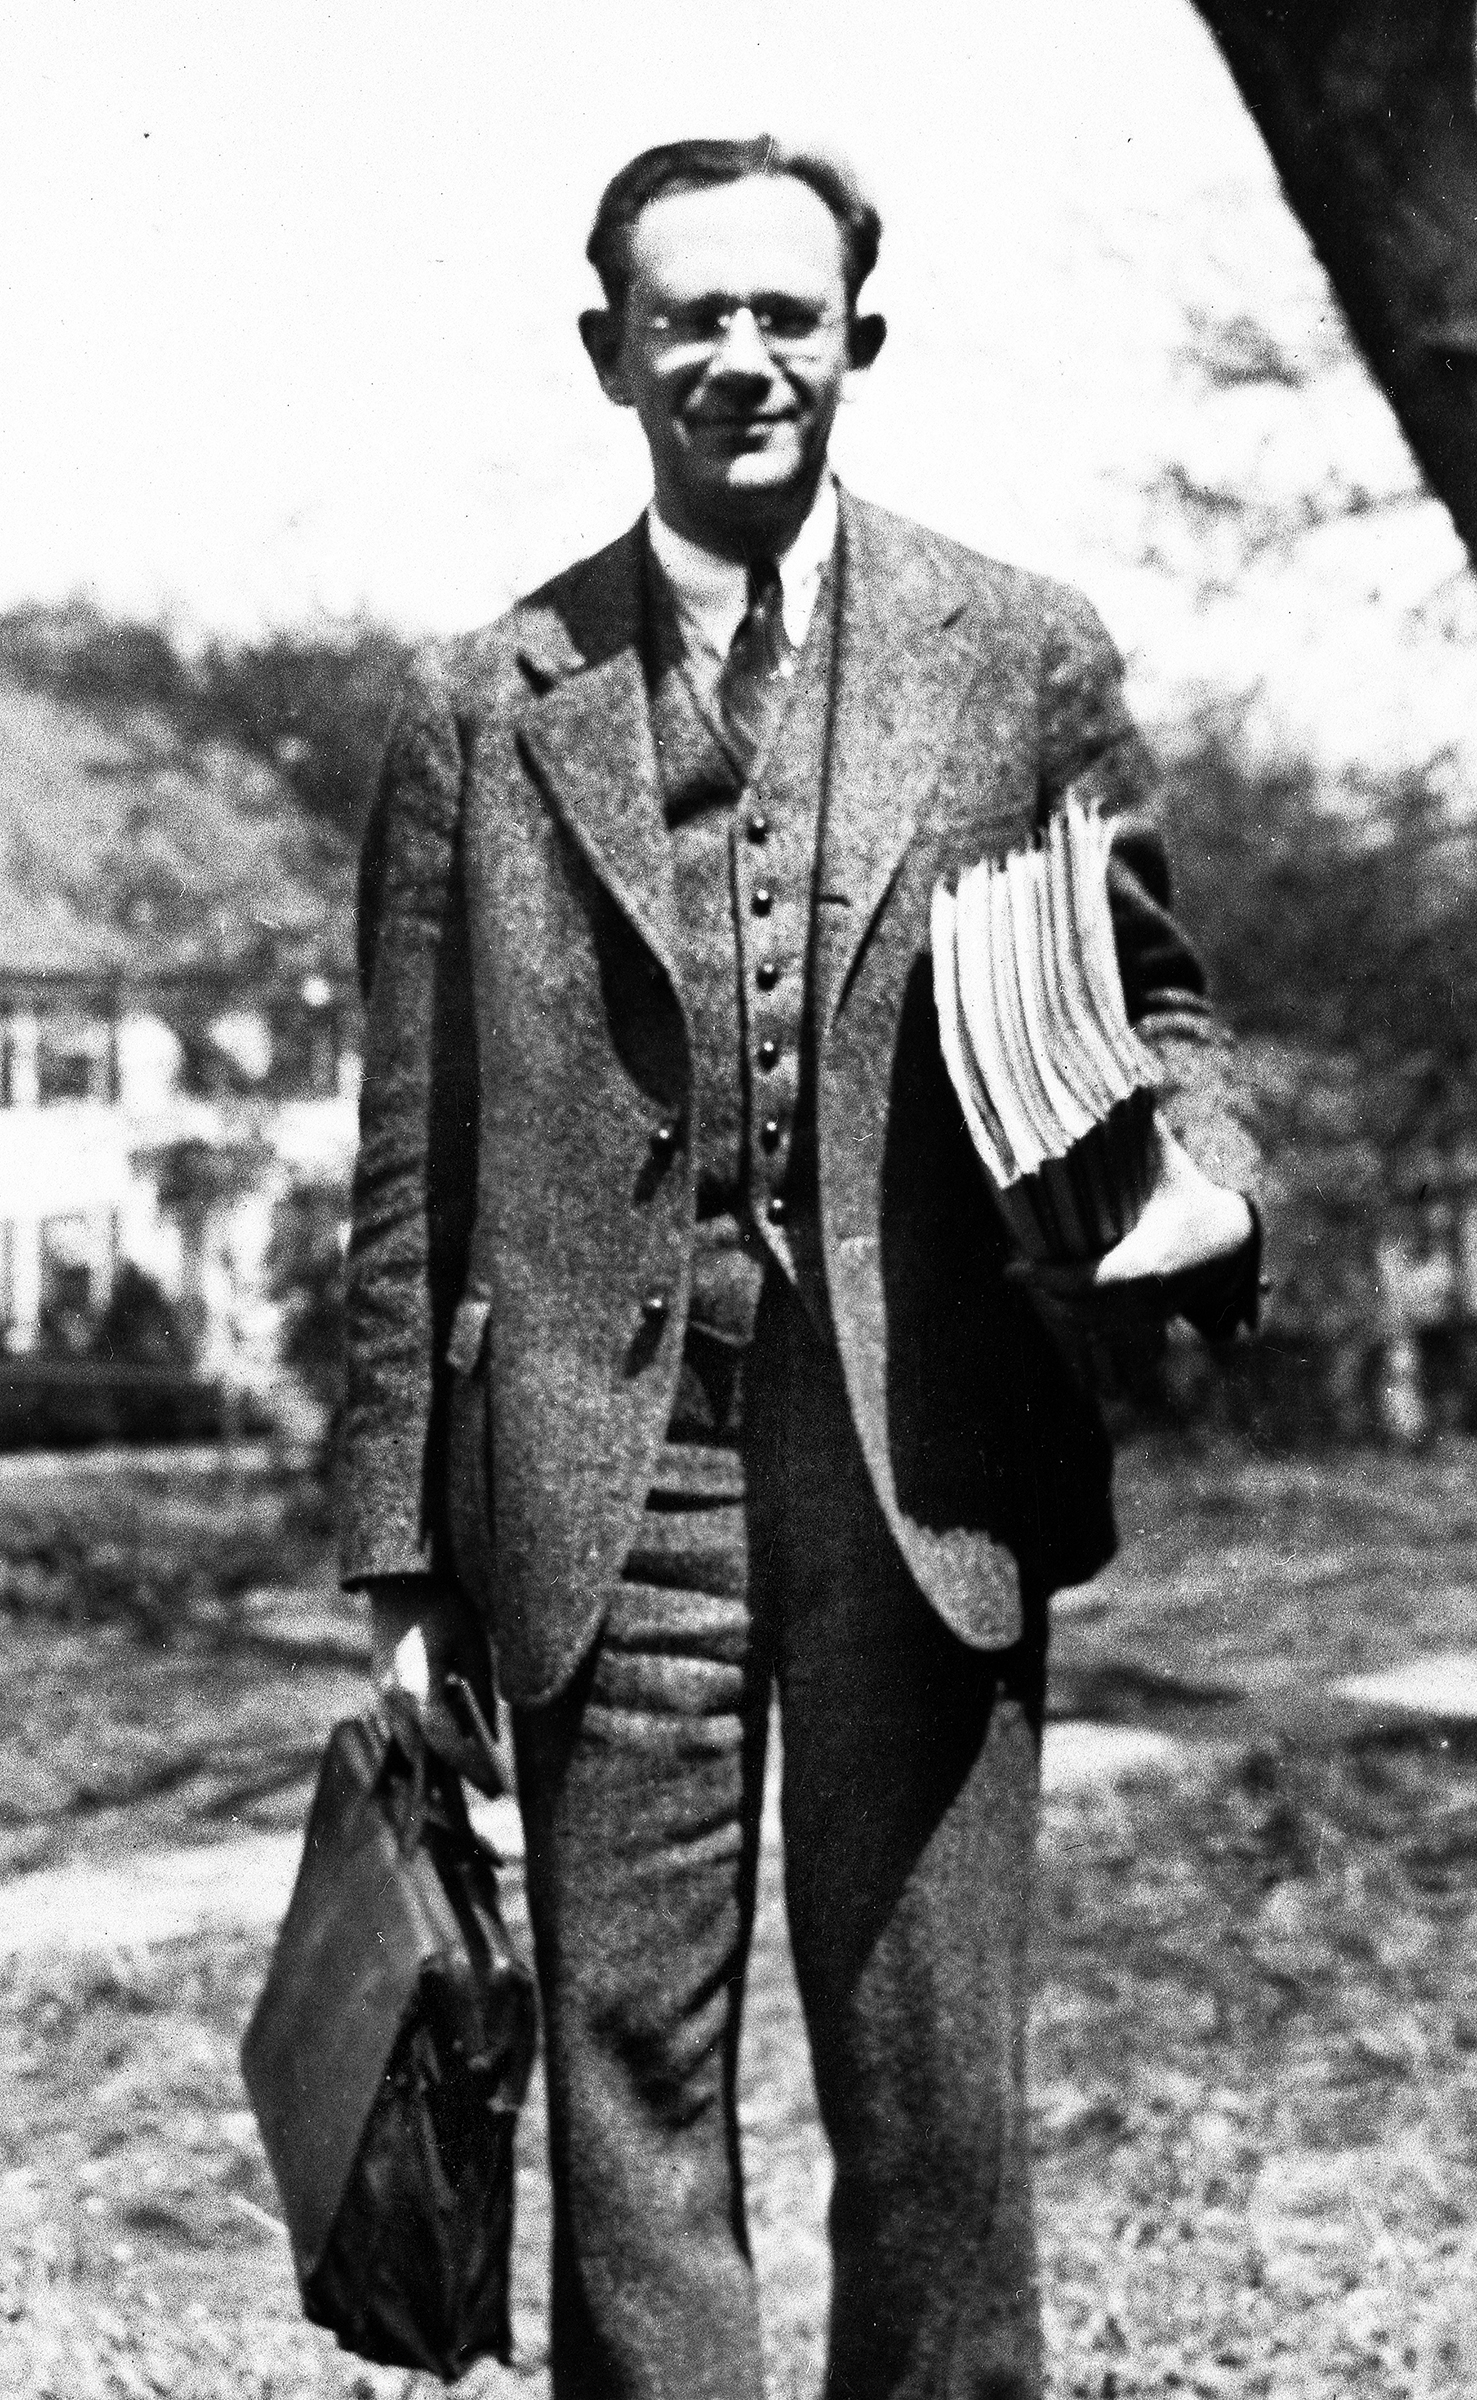
\includegraphics[width=.95\textwidth]{figures/Sapir-Yale.jpg}
  \caption{Edward Sapir (ca. 1938)}
  \label{fig:ch.sapir.sapir_yale}
\end{wrapfigure}
There is no reason to imagine that {\Sapir} simply missed the possibility
of such a solution: his descriptive insight into the language was
clearly quite sufficient to see this analysis, and in fact many of its
ingredients are present explicitly in his description (see, e.g., the
remarks on spirantization as the normal case in
\citealt[63f.]{sapir30:s.paiute}). If he chose to describe this
situation by means of morphological and not phonological properties of
elements, it is likely that some systematic reasoning lay behind the
decision. In fact, it is possible to show that the solutions in the
subsequent literature were not available to {\Sapir} in
principle. Furthermore, it can be shown that his description is in
fact more accurate on empirical grounds than the phonological
alternatives that have been proposed.

We can see immediately that one of these possibilities would not have
been open to {\Sapir}: Harms\ia{Harms, Robert}'s proposal to identify geminating stems by a
final voiceless vowel, as opposed to final voiced vowels in the
spirantizing class. For {\Sapir}, \isi{voicing} of vowels was a property that
was completely predictable, and voiceless vowels were variants (rather
than phonemes). Since an organic representation consists only of
phonemes, it could not contain voiceless vowels, and so Harms\ia{Harms, Robert}'s
solution is excluded. Note that it will not do to say that the
geminating class of morphemes in itself establishes the phonemic
status of voiceless vowels: it remains the case that voiceless vowels
only exist in surface forms under specific, predictable conditions,
and since this generalization remains valid regardless of the
morphological \isi{alternation} in question, voiceless vowels are excluded
in principle from organic \isi{representations}.

I confine my attention, therefore, to \citeauthor{spe}'s proposal
that geminating elements end in an obstruent consonant (which they
suggest is actually \emph{t}, though that is irrelevant to the present
discussion) and \isi{nasalizing} ones in a \isi{nasal consonant}. From {\Sapir}'s
point of view this solution would not have been unacceptable in the
way Harms\ia{Harms, Robert}'s would be, since both obstruents and \isi{nasal consonants} of
course appear in phonemic forms; but there is a different problem.

This is that \ili{Southern Paiute} forms always end in a vowel, and positing
stems and suffixes that end in \isi{consonants} (obstruents or nasals) would
violate what is otherwise an absolutely valid generalization about the
language. This generalization is not true of phonetic forms directly,
since apparently consonant-final words are created by rules of vowel
\isi{devoicing} and subsequent reduction of voiceless vowels or their
absorption into a preceding spirant, or by elision of final short
vowels before a word beginning with a vowel. It is also true that
words may end with a glottal stop; but {\Sapir} argues in his
phonological description that an organic glottal stop is actually
associated with a \isi{syllable} as a whole, and not with a specific
sequential position within it. It may be realized syllable-finally,
but more often is found somewhere within the vowel \isi{articulation}—or
even in a neighboring \isi{syllable}. When these predictable effects are
abstracted away from, however, the generalization remains that
\ili{Southern Paiute} words end in open syllables, and {\Sapir} quite evidently
interprets the same generalization as applying to individual lexical
elements. Morpheme-final obstruents and nasals, then, could not be
posited in phonological forms without violating a canonical pattern of
the language.

The issue which we suggest {\Sapir} implicitly resolved on this basis was
only later raised explicitly. \citet{hale73:lardil} argued that in
several languages, the assumption that a completely general
phonological account should be given for a morphologically limited
phonological pattern leads to incorrect consequences for reasons quite
close to those that apparently motivated {\Sapir}. Strictly speaking, the
discussion of these examples falls outside of the historical purposes
of the present work. Since the issue is one of some significance,
however, and since it can be shown that {\Sapir}'s solution is actually
validated by the evidence from \ili{Southern Paiute} along the same lines as
those argued by Hale, an appendix to the present chapter contains a
further elaboration of these points.

It appears, in fact, that the generalization at work here is of a
piece with other \isi{constraints} imposed in effect on {\Sapir}'s phonological
analyses. The fact noted by {\McCawley} that the set of phonemes
constitutes a subset of the set of surface phonetic segments is
clearly of the same order, since a posited \isi{phoneme} which did not meet
this requirement would violate an obvious generalization about surface
forms. Another instance of the same respect for surface \isi{regularities}
is to be found in the fact that ``any characteristic common to all the
alternants of a morpheme will appear in {\Sapir}'s phonologic
representation of it'' \citep[110]{mccawley67:sapir}. This does not
mean that the phonologic representation is necessarily one of the
occurring surface alternants, of course, or even that all of the
components of such a representation show up in some surface alternant
(e.g., the absolutive suffix in \ili{Southern Paiute} is assigned the
representation \emph{pi}, despite the fact that the initial consonant
always shows up as spirantized \emph{v}, geminated \emph{p:}, or
nasalized \emph{mp}). It does entail, however, that any valid
generalization about the surface form of an element will be reflected
in its \isi{underlying representation}.

In {\Sapir}'s phonology, then, generalizations induced from surface
representation play an essential role in constraining the set of
underlying (`phonemic', `phonologic', `organic') \isi{representations}. Even
though the relation between the two in any particular case may be
quite complex, the two are unified on a global basis across a language
by a single set of \isi{regularities} of distribution and canonical
structure.

Importantly, we should recall that the same set of \isi{regularities} plays
a significant role in determining the class of phonological
rules. These are in general assumed to operate so as to affect
morphologically complex \isi{representations} in which some generalization
would otherwise be violated, so as to make them conform to the
generalization. For example, a language allowing only two-consonant
clusters may insert an epenthetic vowel in the environment
CC{\gapline}C \emph{so as to avoid a cluster of three
  consonants}. This rationale for the existence of \isi{phonological rules},
taken over largely from {\Boas}, serves as the basis of a distinction
between genuinely phonological and (at least partially) morphologized
rules for {\Sapir}.

The features of {\Sapir}'s practice which have most often been noted are
the distance between his \isi{underlying representation}s and surface
phonetics, and the role played by rules of \isi{alternation} (formulated as
replacement processes) in his grammars. To understand the central
points of his analyses, however, it is important to see that both of
these components of an analysis are construed by him as organized by
the \isi{regularities} obtaining in surface forms. The elements of
\isi{phonological representations} are determined by reference to rules of
the language: as observed above, the natural classes and
linguistically significant affinities among phonemic elements are
given by the \isi{regularities} of distribution and \isi{alternation} that they
participate in. Conversely, the \isi{phonological rules} of the language
function primarily to maintain a regularity determinable from the
canonical form of surface \isi{representations}. Few linguists,
historically, have held as unified a view as {\Sapir} of the
interrelationship of considerations of rules and \isi{representations} in a
single structure within natural languages. In some ways, however,
{\Sapir}'s use of surface \isi{regularities} to drive other aspects of a
language's phonology anticipates the central role of \isi{constraints} on
surface form in \isi{Optimality Theory}, an approach we consider in
chapter~\ref{ch.otlabphon}.

\newpage
\begin{figure}
  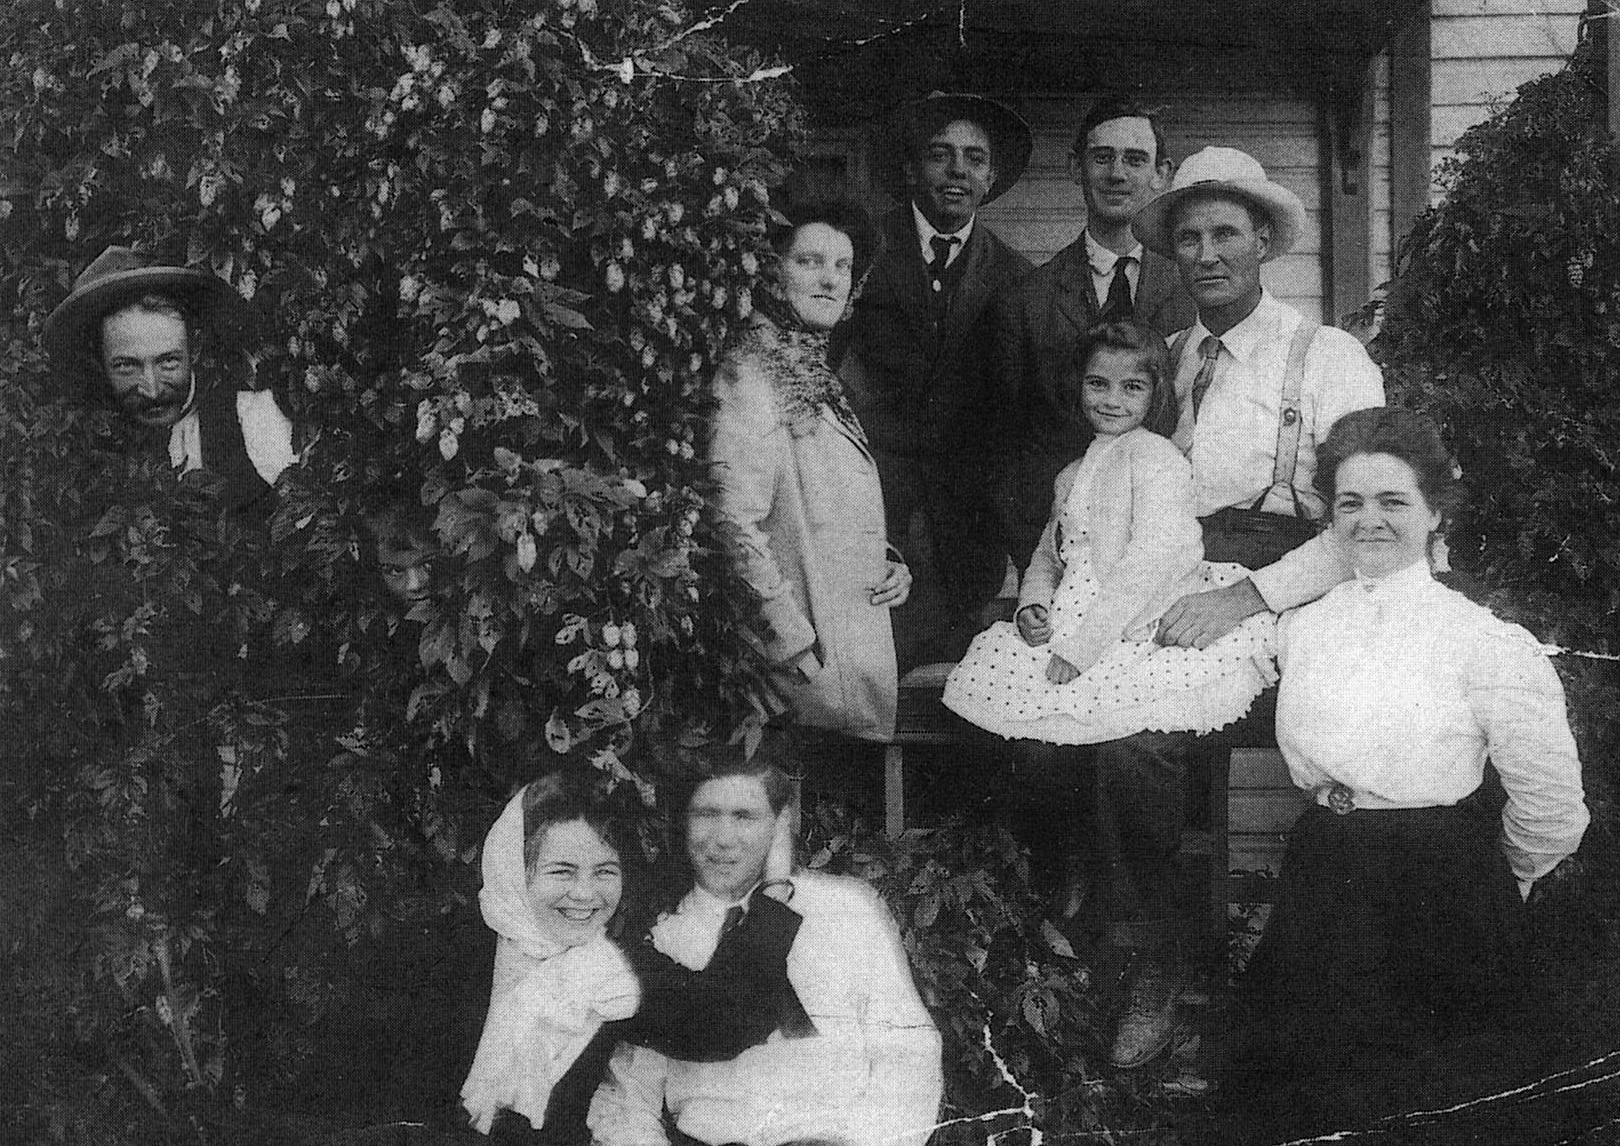
\includegraphics[width=.75\textwidth]{figures/Sapir-utes.jpg}
  \caption{Edward Sapir (1909) {[In glasses, with group at
      Mrs. Dodd's, Uintah Ute Reservation, White Rock, Utah.  J. Alden
      Mason peering from bushes]}}
  \label{fig:ch.sapir.sapir_utes}
\end{figure}

\section*{APPENDIX: Abstractness and {\Sapir}'s analysis of Southern
  Paiute}
\addcontentsline{toc}{section}{APPENDIX: Abstractness and Sapir's analysis of Southern
  Paiute}

A central feature of {\Sapir}'s analysis of \ili{Southern Paiute} is his claim
that the spirantizing, \isi{nasalizing}, or geminating effect of stems (and
affixes) on a following affix is to be stated as a morphological
property of individual elements, rather than in terms of
phonologically derived consequences of the elements' underlying
shape.  The most plausible alternatives to that analysis
discussed above all involve positing underlying shapes that violate an
otherwise valid generalization about the language—that words (and thus
stems) do not end in \isi{consonants}. They would thus be inconsistent with
{\Sapir}'s overall approach to phonological structure.

A set of similar cases are discussed by \citet{hale73:lardil},
including a particularly clear example furnished by the phonology of
several languages of the Polynesian family. Hale\ia{Hale, Kenneth}'s discussion is based
on Māori, but we take our examples below from Sāmoan, where the facts
are quite similar, but somewhat more complex and revealing.  In Sāmoan
(as in Māori) there are no consonant clusters, and no final
\isi{consonants}; i.e., all syllables are open. There is very little
inflectional morphology in the language, but most verbs have a
so-called `passive' form, and many have a plural, reciprocal, and/or a
gerund form in addition. The passive is almost always formed by the
addition of a suffix which is the reflex of proto-Polynesian
*-\emph{C-ia}, where the particular consonant that appears differs from
one verb to another. Thus, \emph{o'o} `arrive, reach' has the passive
\emph{o'otia}, but \emph{oso} `jump', passive \emph{osofia};
\emph{ula} `make fun of', passive \emph{ulagia},\footnote{Sāmoan
  \emph{g} = [ŋ].} \emph{inu} `drink', passive \emph{inumia},
etc. Since the consonant that appears in the suffix depends on the
root that is involved, the lexical entry for a root must contain some
indication of which form the suffix takes when added to it.

There are evidently two basic alternatives open for the description of
these facts. We might follow {\Sapir}'s example in his \ili{Southern Paiute}
and characterize each stem with an abstract morphological operator:
thus, the phonological representation of \emph{o'o} would be simply /o'o/,
with the additional indication that it is a `\emph{t}-stem' (as opposed to
/oso/, which is an `\emph{f}-stem', etc.). In this case, the suffix itself
would have several morphologically determined forms: /-tia/ with some
verbs, /-fia/ with others, etc.

Alternatively, we might incorporate the suffix consonant into the
representation of the stem itself, giving \isi{underlying representation}s
such as /o'ot/, /osof/, etc. In this case, the suffix could be given a
unitary underlying form /-ia/; and the correct forms could be derived
simply by the application of a rule deleting final \isi{consonants} when no
suffix follows. On that basis /o'ot/ would yield surface [o'o], but
/o'ot+ia/ would give [o'otia] since the truncation rule would not
apply in this form. This second solution involves no arbitrary
morphological features, and only a single completely automatic
phonological rule (final consonant truncation). It is evidently
simpler from a purely formal point of view than the morphological
account; and it is noteworthy that when \citet[219]{bloomfield:lg}
discusses this example, he adopts that analysis without further
comment, as if it were obvious. This is also an example frequently
used in elementary linguistics classes, since the phonological account
of the \isi{variation} is so easy to arrive at and may well represent the 
historical development.

Nonetheless, there are some problems for this solution. From a purely
phonological point of view, the fact that some suffix variants are not
simply -\emph{Cia} poses a slight problem: the forms -\emph{ina}
(e.g. \emph{salu} `sweep', passive \emph{saluina}), -\emph{a}
(e.g. \emph{ave} `take', passive \emph{avea}), and -\emph{na}
(e.g. \emph{'ai} `eat', passive \emph{'aina}) are not
straightforwardly derivable from some stem form plus /-ia/. Assuming
we ignore these as simply suppletive forms of the suffix, there still
remain more serious difficulties.

For instance, the causative form of verbs is made with the prefix
\emph{fa'a-}, sometimes with \isi{reduplication} of the root. Interestingly,
virtually all such causatives take the passive suffix /-ina/,
regardless of the suffix taken by the noncausative: e.g., \emph{pa'u}
`fall' has the passive \emph{pa'utia} indicating that its stem-final
consonant (on the phonological solution) should be /t/, but its
causative \emph{fa'apa'u} has the passive
\emph{fa'apa'uina}. Similarly, \emph{manatu} `remember' has the
passive \emph{manatua}, but its causative\emph{ fa'amanatu} `remind'
has the passive fa'\emph{amanatuina}. The stem \emph{oso} `jump'
apparently ends in /-f/, if this is what is indicated by the passive
\emph{osofia}; but in that case the causative \emph{fa'aosooso} is
doubly problematic: first because the supposed final /-f/ is not
preserved before the reduplicated copy (i.e., the causative is not
*\emph{fa'aosofoso}); and second because its passive is
\emph{fa'aosoosoina} (not *\emph{fa'aosoosofina}).

It might be claimed that the causative morphology involves truncating
the final consonant and then replacing the passive ending appropriate
to the root with another; but aside from the fact that this seriously
weakens the explanatory force of the proposed final consonant in the
phonological form, it will still not resolve all difficulties. In
addition to the passive, Sāmoan also has another suffix (the
reciprocal), which usually takes the form -\emph{C(a')i} with
different \isi{consonants} depending on the root. Forms such as
\emph{fe-ita-ga'i}, reciprocal of \emph{ita} `be angry', appear to
lend support to the final consonant solution, since the passive of
this stem is \emph{ita-gia}: the two show the same idiosyncratic
consonant, a fact which is immediately explained if this consonant is
part of the stem. But in that case, forms such as \emph{alofa} `love'
pose a problem: its passive is \emph{alofa-gia}, but its reciprocal is
\emph{fe-alofa-ni}. In such a case there is apparently no single form
of the stem which can account for all variants.

\citet{hale73:lardil} cites similar facts from Māori, together with a
number of generalizations about the direction of regularization
through \isi{historical change}, to argue that despite the \isi{simplicity} of the
phonological solution, the descriptively adequate account of this
\isi{variation} is actually the morphological one. Most importantly for our
purposes, he argues that in this case (and in other unrelated ones
which he examines), the morphological solution is to be preferred for
a principled reason: because the phonological solution posits
underlying forms (with final \isi{consonants}) which violate an important
surface generalization about the language (all syllables are open),
this disparity between the canonical forms of deep and surface
\isi{representations} excludes the phonological solution altogether. I have
argued above that it is exactly this consideration which (at least in
part) led {\Sapir} to prefer a morphological account in \ili{Southern Paiute}:
phonological \mbox{(near-)}surface forms always end in vowels, so it is not
acceptable to posit underlying forms that violate this generalization
by ending in obstruent or \isi{nasal consonants}.

If {\Sapir} was thus influenced in choosing a morphological analysis of
the consonant alternations in \ili{Southern Paiute} by considerations like
those noted by Hale, this would still not be an empirical argument for
his solution, and it is especially important (if we are interested in
the correctness of the theory) to ask whether there is additional
evidence bearing in the same direction. In fact, when we examine the
phonology and morphology of \ili{Southern Paiute} (and {\Sapir}'s description
of it) more closely, there turn out to be important problems for the
phonological view which also argue in favor of the morphological
account.

In his discussion of why he adopts the morphological position, {\Sapir}
notes that there is no independently motivated difference in the
phonological shape of spirantizing, geminating, and \isi{nasalizing} stems
to which their differential behavior could be related. Of course, that
is just what is in question; and the claim of the phonological account
is precisely that there is such a difference, but that it is
neutralized if no suffix which would allow it to surface follows the
stem. {\Sapir} argues on the basis of comparative data that there is no
consistent etymological difference either, which would not of course
bear directly on the synchronic descriptive issue (though it is
strongly suggestive of a non-phonological account if one believes
phonological alternations are usually, if not always, the reflex of
\isi{historical change}).

Much more significant than the sort of plausibility argument one might
found on historical considerations, however, are the purely
descriptive problems which a phonological account must face. Recall
that on that view, suffixes are uniformly represented with simple
\isi{consonants}, and the spirantized, geminated, and nasalized alternants
arise by virtue of the effect of a stem-final vowel, obstruent, or
nasal on this segment. This assumes that the suffix shapes appearing
with particular stems are exclusively a function of a unitary
underlying phonological property of stems.

There are a number of suffixes, however, which have \isi{invariant} forms,
regardless of the character of the stem they are attached to. Some of
these are consistently nasalized (e.g., \emph{-ŋqï-} `Indirective,
\emph{to}, \emph{for}'); some geminated (e.g. \emph{-q:u-} `numeral
objective'), and some invariably spirantized (e.g.,
\emph{-γa-}`durative'). On one version of a strictly morphological
account, all that would need to be said about these items is that
their lexical entries have only a single phonetic form corresponding
to their organic form: this has the effect of blocking the
morphologically conditioned selection of non-occurring variants. On the
phonological account, however, one must introduce additional rules:
for example, to eliminate a posited underlying stem-final nasal or
obstruent consonant before a suffix which is invariantly spirantized.

A number of other suffixes appear in two of the three possible forms,
but not in the third. In general, these appear either spirantized or
nasalized but not geminated. After geminating stems these elements
occur spirantized: for example, the agentive suffix \emph{-vi/-mpi}
has no geminate form, and thus appears spirantized after the
geminating stem \emph{nɔ:-} `to carry on one's back' (in
e.g. \emph{niŋwï'-nɔ˙$^{\textit{ɔ}}$-ϕɪ} `person-carrier, mythical
bird that carries people away in its talons'). {\Sapir} traces the
nasalized variants of these suffixes to an independent phonological
rule of nasalization applying after a nasal in the preceding \isi{syllable}
(as in the future suffix \emph{-vania}, appearing as \emph{-mpania} in
\emph{iviŋumpania} `will take a drink'). This process is distinct from
morphological nasalization, which does not require a \isi{nasal consonant}
in a \isi{nasalizing} element: for example, the stem \emph{pa'a-} `to be
high' and the suffix \emph{-vi} `agentive', among others, are
\isi{nasalizing} despite the lack of a \isi{nasal consonant} in their phonological
form. {\Sapir} thus treats the nasalization of the `two-shape' suffixes
as extraneous, and reduces the issue to a difference between forms
that undergo the morphological processes of consonant \isi{alternation} and
those that do not. A problem is posed for this account, however, by
the fact that such suffixes appear nasalized after even those
\isi{nasalizing} stems that contain no \isi{nasal consonant}: \emph{paγimpani} `I
shall go', from \isi{nasalizing} \emph{paγi-} `go, walk' plus the future
suffix \emph{-va/-mpa}.

In order to describe the exceptional items on the purely phonological
account, it must be assumed either that they undergo spirantization
even after obstruents or that they trigger exceptional deletion of a
preceding obstruent (but not of a nasal). One interpretation of
{\Sapir}'s morphological account, in \isi{contrast}, simply involves omitting a
geminated alternant from the lexical entry: the nasalized form will be
chosen correctly where appropriate, with the spirantized form treated
as the `elsewhere' case.

Some of these exceptional suffixes simply represent specialized uses
of one of the variants of a \isi{regular}, alternating suffix. The suffixes
\emph{-γi} `to come in order to {[---]}' and \emph{-γwa'ai} `to go in
order to {[---]}', for example, are invariantly spirantized. They are
clearly related, however, to the alternating suffixes
\emph{-γi/k:i/ŋki} `to come while {[---]}ing' and
\emph{-γwa'ai/k:wa'ai/ŋkwa'ai} `to go while {[---]}ing'. To describe
this phonologically, we must assume the suffix acquired a special
sense together with the necessary exception features to enforce
spirantization even after consonant-final stems; but if we take
{\Sapir}'s account, we need only say (as he does) that one of the
existing variants of the \isi{regular} suffix acquires a special sense.

Just as the description of the suffixes poses problems for the
phonological account, a consistent description of the stems also seems
difficult on that view. For example, the same stem may well appear
with one suffix variant in some cases but with another in others:
e.g., \emph{wa'a} `cedar' is normally geminating, as shown by
\emph{wa'ap:ï} `cedar tree', but sometimes takes nasal suffixes as in
\emph{wa'ampi} `cedar berry'. To describe such cases, we would have to
assume the stem has two distinct phonological shapes, distributed on a
morphologically determined basis.

In this same vein, there is an interesting semisystematic tendency for
spirantizing stems to be treated as geminating when they are
compounded with other independent stems: e.g., \emph{aŋqa-} `red' is
normally spirantizing, as shown by \emph{aŋqaγa} `to be red', but
often appears as geminating in compounds like \emph{aŋqap:aγi} `red
fish, trout' or \emph{aŋqa-q:ani} `red house'. {\Sapir} notes that the
tendency to use geminate variants of stems in compounds may be due to
the greater phonetic similarity between this form and the (initial,
thus unspirantized) consonant of the simplex form; for discussion, see
\citealt{darden84:s.paiute}.

For our purposes, the interesting point is that {\Sapir} sees this
restructuring as ``the first step towards the dulling of a
consciousness of consonantal alternations and toward their development
into mere historical survivals'' \citep[70]{sapir30:s.paiute}. He
envisions a developmental sequence similar to that posited by 
{\DeCourtenay} and {\Kruszewski} (see above, chapter~\ref{ch.kazan}), by
which a process which may once have been phonological has become
morphological, and is on its way to becoming a merely lexical
relic. If we assume the phonological view, we must claim that the
unusual behavior resides not in the second element of such compounds,
where {\Sapir} plausibly localizes it, but rather in the development of
irregular obstruent-final variants of the first elements—variants
which only appear compounded.

None of this evidence demonstrates conclusively that a phonological
account of the \ili{Southern Paiute} suffix \isi{alternation} is
\emph{impossible}; rather (like Hale\ia{Hale, Kenneth}'s evidence from Māori and the
similar facts reviewed above from Sāmoan), the evidence indicates that
it is less appropriate than the morphological analysis pursued by
{\Sapir}.

Further evidence derived from the facts of \isi{reduplication} makes
this case even clearer. Reduplication normally copies the initial CV
of an element; e.g., \emph{sivai} `whittles' reduplicates as
\emph{sisivai} `whittles many times'. The stem consonant following the
reduplicated \isi{syllable} is no longer word-initial and thus subject to
change, and the changes it undergoes are the same three as those found
in suffix \isi{alternation}: spirantization, gemination, or
nasalization. Since the shape of the stem is more self-evident than
the identity of a hypothetical stem-final consonant, the facts of
\isi{reduplication} ought to provide clear evidence for whether or not
phonological structure is the essential determinant of these
alternations.

Cases in which \isi{reduplication} results in nasalization appear to provide
some evidence in favor of the phonological account, because most of
these are stems of the shape /CVNX/ (e.g., \emph{qani} `house', which
reduplicates as \emph{qaŋqani} `houses'). If we allowed the
\isi{reduplication} rule to copy CV(N), instead of only CV, and treated
nasalization as resulting from a sequence of \isi{nasal consonant} plus
stop, this result would follow directly. Unfortunately, however, there
are some instances in which \isi{nasalizing} \isi{reduplication} arises without a
\isi{nasal consonant} in the stem ({\Sapir} cites \emph{pɔmpɔtsats-} `lizard'),
which suggest that nasalization in \isi{reduplication} (though largely
predictable) is in part morphologized.

The case of geminating \isi{reduplication} is much more difficult to explain
phonologically. The class of stems that geminate when they reduplicate
seems completely unpredictable: thus, although \emph{tava'c:upï }`dry'
reduplicates as \emph{t{\scriptsize A}ta'ϕ{\scriptsize A}cupï:} `all
dry' with a geminate,  \emph{tavin'na} `put out one's breast,
strut' reduplicates as \emph{tara'vin'naai} `keeps putting out (his)
breast' with a spirantized form. It should be emphasized that there is
no consistent correlation between the form CVCX where the second C is
an obstruent (or a geminate) and geminating, rather than spirantizing
\isi{reduplication}.

Further, the gemination may affect a stem-internal consonant, rather
than a stem initial one: e.g., \emph{ivi} `drink' reduplicates as
\emph{i'ip:i} `drinks repeatedly' with a geminate, or
\emph{tïv\textsuperscript{w}ïn:aγai} `leads', as \emph{tï'tïp:ïnaq:ai}
`leads away several times'. Finally, the same stem may appear with
more than one kind of \isi{reduplication}, in different morphological
categories. The stem \emph{qwïï-} `take' forms a distributive
\emph{qwïγwïï} `several take (one object)' with spirantizing
\isi{reduplication}, but also an iterative qwï'qwïï `to take one object
several times'. All of these facts indicate that morphological factors
and not phonological structure determine the applicability of the
process of `gemination'.

We conclude, then, that a variety of evidence suggests that {\Sapir} was
right in treating the spirantizing, geminating, and \isi{nasalizing}
processes in \ili{Southern Paiute} as morphologically rather than
phonologically conditioned. This result is of some interest in itself,
but we have pursued it at such length here not simply as a matter of
descriptive linguistics. Rather, the point to be made is that a
phonological solution (if correct) would have been available to {\Sapir},
if systematic considerations had not led him to prefer the
morphological account. These systematic factors, we suggest, are the
same as those discussed by \citet{hale73:lardil}: a desire to avoid
positing underlying forms which would violate a basic generalization
about the structure of surface forms in the language.

%%% Local Variables: 
%%% mode: latex
%%% TeX-master: "/Users/sra/Dropbox/Docs/Books/P20C_2/LSP/main.tex"
%%% End: 

